
\section{General Remarks}

\subsection{Treatment Sensitivity Prediction for Personalized Medicine}

The goal of personalized medicine is to provide custom-tailored medicine
to every patient. An essential part of this is to select an appropriate
treatment for a specific patient out of the available treatments.
The treatment should have a high probability of succeeding. One way
of approaching this is through machine learning on the expression
data from a patient's tissue to predict treatment outcome. Such a
prediction requires similar expression data from multiple patients
that already underwent the treatment and where the therapy outcome
is known.

In order to evaluate the usefulness of deep learning in the context
of personalized medicine, we analyzed a data set that had something
to do with drug sensitivity and resistance. GSE25055 and GSE25065
are microarray expression data sets produced for the same paper, namely
\cite{HatzisSymmans2011}. Table \ref{tab:GSE25055-GSE25065-sample-number}
shows the number of samples of each label in both data sets. The authors
used GSE25055 to generate a classifier for the prognosis of breast
cancer patients that received reductive surgery preceded by taxane-anthracycline
chemotherapy. All patients had ERBB2 (also called HER2 or HER2/neu)-negative
breast cancer. From each patient, tissue was extracted in reductive
surgery and measured for genome-wide gene expression on Affymetrix
HG-U133A microarrays. 

After an observation period of a couple of years, the mean of which
was 3 years, the patients were labeled as either showing \emph{pCR}\index{pCR}
or \emph{RD}\index{RD} to chemotherapy. \emph{pCR }is an abbreviation
of \emph{pathologic complete response}\index{pathologic complete response}
and means that there was no sign of a remaining breast cancer. In
the following it will be labeled as ``class 1'' or ``label 1''.
\emph{RD} abbreviates \emph{residual disease}\index{residual disease}
and means there was still cancerous tissue. It will be termed ``class
0'' or ``label 0''.

\cite{HatzisSymmans2011} then tested their classifier on an independently
measured data set, GSE25065. The input to the prediction was the expression
data and the desired output a label of either \emph{RD }or \emph{pCR}.

\begin{table}
\begin{centering}
\begin{tabular}{|c|c|c|c|c|}
\hline 
 & label 0, RD & label 1, pCR & label NA & $\sum$\tabularnewline
\hline 
\hline 
GSE25055 & 249 & 57 & 4 & 310\tabularnewline
\hline 
GSE25065 & 140 & 42 & 16 & 198\tabularnewline
\hline 
\end{tabular}
\par\end{centering}
\caption[Number of samples in GEO datasets GSE25055 and GSE25065.]{\label{tab:GSE25055-GSE25065-sample-number}Number of samples in
GEO datasets GSE25055 and GSE25065. ``label 0, RD'' means ``residual
disease''; ``label 1, pCR'' means ``pathologic complete response''.
``label NA'' means that microarray data for the patient is available,
but not his/her disease status.}
\end{table}

\subsection{Goal of this Work}

The context of this work is the use of classifiers on high-dimensional
data as supporting tools for treatment decisions. Three types of neural
networks that lend themselves to semi-supervised training were used:
autoencoders, Restricted Boltzmann Machines and Deep Belief Networks.
Parallel to these, the performance of a semi-supervised version of
Support Vector Machines, namely the Transductive SVM was evaluated.

The specific goals were:
\begin{enumerate}
\item to find out whether incorporating unlabeled expression data in the
training of deep artificial neural networks enhances a classifier's
performance.
\item to assess performance of the classifier on an independently measured
data set.
\item to evaluate whether artificial neural networks can compete with established
classification algorithms like SVMs.
\end{enumerate}

\subsection{How Unlabeled Data Was Used in Training}

In the following, we will discuss how we used unlabeled data in semi-supervised
training.

\subsubsection{How Unlabeled Data was Used in Pre-Training Autoencoders and Fine-tuning
Using Back-propagation}

Autoencoders\index{autoencoder} are composed of an encoder\index{encoder}
and a decoder\index{decoder}. The encoder tries to compress the input
data and the decoder tries to reconstruct the input from its compressed
form. Training autoencoders is unsupervised. As a general rule only
the samples designated as ``unlabeled'' were used in training the
unsupervised part of an algorithm.

The decoder network of the trained autoencoder was then discarded,
so that only the encoder remained. Classification was done on the
compressed representation of the input. The classifier network was
built on top of the encoder (see figure \ref{fig:supervised-network-on-top-of-unsupervised}),
and the compressed output layer of the encoder was used as the input
layer of the classifier.

\begin{figure}
\begin{centering}
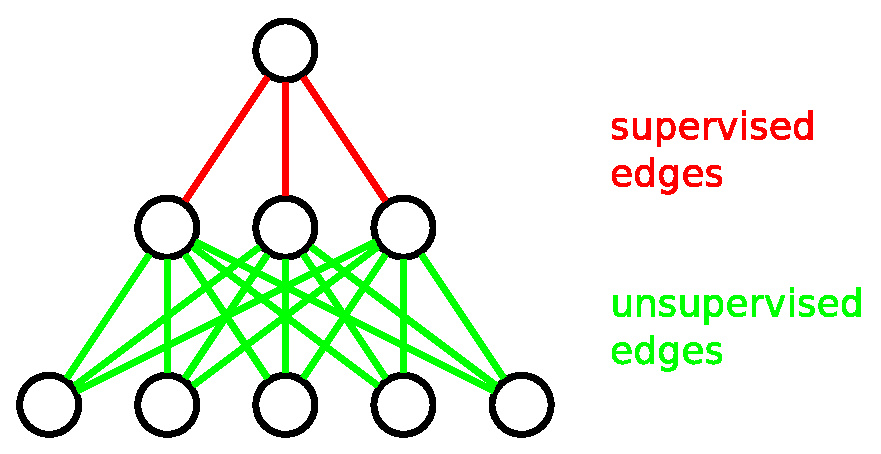
\includegraphics[width=0.35\paperwidth]{images/progress_report_201411-unsupervised-to-supervised}
\par\end{centering}
\caption[How a supervised network is trained on top of a pre-trained unsupervised
network.]{\label{fig:supervised-network-on-top-of-unsupervised}Example scheme
showing how the supervised network is trained on top of a pre-trained
unsupervised network. The network receives input from the bottom,
and the resulting label is read off at the top. The unsupervised network
can be more than 2 layers deep. It is trained first during pre-training.
Then the supervised network is appended onto the top and trained together
with the unsupervised network.}
\end{figure}

The weights of the classifier were initialized randomly, and standard
back-propagation was used to train the whole network to classify samples.
Hence, the encoder can be modified by back-propagation training, but
pre-training with the autoencoder initializes it to a configuration
that ``knows'' about the unlabeled samples. The learning rate of
the second training run (\emph{fine-tuning}\index{fine-tuning}) should
be small enough not to diverge from the unlabeled training configuration
in too large steps (per iteration).

Algorithm \ref{alg:pretrain-autoencoder-finetune-backprop} shows
the pseduo-code for pre-training using a DBN and fine-tuning using
backpropagation.

\begin{algorithm}
\begin{enumerate}
\item initialize the autoencoder $A$
\item \label{enu:Autoencoder-for-all-unlabeled-training-data}for all unlabeled
training samples $U$ in the unlabeled training data set:

\begin{enumerate}
\item set the input of $A$ to $U$
\item train $A$ with the goal of reconstructing $U$
\end{enumerate}
\item repeat step \ref{enu:Autoencoder-for-all-unlabeled-training-data}
until the reconstruction error is small enough
\item replace the decoder part of $A$ with a randomly initialized classifier
to form the feed-forward network $C$
\item \label{enu:Autoencoder-for-all-training-pairs}for all labeled training
data, consisting of input samples $X$ and corresponding desired output
sample $Y$ :

\begin{enumerate}
\item set the input of $C$ to $X$
\item train $C$ using back-propagation to output $Y$
\end{enumerate}
\item repeat step \ref{enu:Autoencoder-for-all-training-pairs} until the
classification error is small enough (subject to early stopping or
model selection)
\end{enumerate}
\caption{\label{alg:pretrain-autoencoder-finetune-backprop}Pre-training on
unlabeled data using an autoencoder and backpropagation fine-tuning
with labeled data.}
\end{algorithm}

\subsubsection{How Unlabeled Data was Used When Pre-training a Restricted Boltzmann
Machine and Fine-tuning Using Back-propagation}

When using the unsupervised Restricted Boltzmann Machine to find the
approximate weights of a neural network, the unlabeled data were used
to train the Restricted Boltzmann Machine. The resulting neural network
was then extended with the network layer for supervised classification,
and the complete network was trained using (supervised) back-propagation
on the labeled data. 

Algorithm \ref{alg:pretrain-RBM-finetune-backprop} shows the pseduo-code
for pre-training using a DBN and fine-tuning using backpropagation.

\begin{algorithm}
\begin{enumerate}
\item initialize the Restricted Boltzmann Machine $R$
\item \label{enu:RBM-for-all-unlabeled-training-data}for all unlabeled
training samples $U$ in the unlabeled training data set:

\begin{enumerate}
\item train $R$ with the goal of learning the probability distribution
of $U$
\end{enumerate}
\item repeat step \ref{enu:RBM-for-all-unlabeled-training-data} until the
reconstruction error is small enough
\item put a classifier on top of $R$ to form the feed-forward network $C$
\item \label{enu:RBM-for-all-training-pairs}for all labeled training data,
consisting of input samples $X$ and corresponding desired output
sample $Y$ :

\begin{enumerate}
\item set the input of $C$ to $X$
\item train $C$ using back-propagation to output $Y$
\end{enumerate}
\item repeat step \ref{enu:RBM-for-all-training-pairs} until the classification
error is small enough (subject to early stopping or model selection)
\end{enumerate}
\caption{\label{alg:pretrain-RBM-finetune-backprop}Pre-training on unlabeled
data using a Restricted Boltzmann Machine and backpropagation fine-tuning
with labeled data.}
\end{algorithm}

\subsubsection{How Unlabeled Data was Used in Training Deep Belief Networks}

Deep Belief Networks are an unsupervised algorithm and thus were trained
using unlabeled data. As with Restricted Boltzmann Machines, the
resulting network was then extended with the classifier layer, and
the complete network was fine-tuned using back-propagation on the
labeled data.

Initializing the complete network with the weights and biases of a
trained DBN serves the purpose of initializing the complete network
to a low energy configuration that has a higher chance to be trainable
using back-propagation. It does not prevent back-propagation from
settling in a configuration that is far away from the weights and
biases of the trained DBN.

Algorithm \ref{alg:pretrain-DBN-finetune-backprop} shows the pseduo-code
for pre-training using a DBN and fine-tuning using backpropagation.
It is identical to pre-training using a Restricted Boltzmann Machine
and fine-tuning using back-propagation, except that we pre-train the
$n$ layers of the Deep Belief Network using RBMs on re-represented
data.

\begin{algorithm}
\begin{enumerate}
\item initialize the Deep Belief Network $D$ to a Restricted Boltzmann
Machine with visible and hidden layer sizes equal to the first two
layers of the DBN
\item for layer $l=2\ldots n$ in the Deep Belief Network:

\begin{enumerate}
\item \label{enu:DBN-for-all-unlabeled-training-data}for all unlabeled
training samples $U$ in the unlabeled training data set:

\begin{enumerate}
\item set re-represented data $R$ to the representation of $U$ in layer
$l-1$
\item think of layers $l-1$ and $l$ in $D$ as a Restricted Boltzmann
Machine and train it with the goal of learning the probability distribution
of $R$
\end{enumerate}
\item repeat step \ref{enu:DBN-for-all-unlabeled-training-data} until the
reconstruction error is small enough
\end{enumerate}
\item put a classifier on top of $D$ to form the feed-forward network $C$
\item \label{enu:DBN-for-all-training-pairs}for all labeled training data,
consisting of input samples $X$ and corresponding desired output
sample $Y$ :

\begin{enumerate}
\item set the input of $C$ to $X$
\item train $C$ using back-propagation to output $Y$
\end{enumerate}
\item repeat step \ref{enu:DBN-for-all-training-pairs} until the classification
error is small enough (subject to early stopping or model selection)
\end{enumerate}
\caption{\label{alg:pretrain-DBN-finetune-backprop}Pre-training on unlabeled
data using a Deep Belief Network and backpropagation fine-tuning with
labeled data.}
\end{algorithm}

\subsection{Issues in Running \emph{deepnet}}

\emph{deepnet} is a neural network implementation written by Nitish
Srivastava, which uses a matrix library (called cudamat) written by
Vlad Mnih and Alex Krizhevsky \cite{Deepnet2014}. It can run on graphics
cards (supporting CUDA). Since graphics cards have a highly parallel
architecture, training times are faster. However, because graphics
cards have to process large data, their RAM is more expensive than
normal RAM for PCs. The graphics cards used have 4 GB of RAM installed.
\emph{deepnet} loads all data sets onto the graphics card at the beginning
of the computation. In addition, the parameter matrices have to be
held in memory. However, there is another matrix library (called
eigenmat and with the same interface as cudamat), which runs on the
normal floating-point unit of a normal CPU. Most of the data sets
were trained on a computer that has 256GB of RAM and 32 cores, which
was more than enough for the data sets tested. There was a bug in
this library when run on 64-bit CPUs, which we fixed. The deepnet
version used can be downloaded from \href{https://github.com/moa1/deepnet/tree/nnet}{https://github.com/moa1/deepnet/tree/nnet},
revision 963C.

\subsection{Training Iterations and Evaluations}

We trained both the unsupervised as well as the supervised network
for a pre-determined number of iterations. This number was determined
by a trial training run on the data set in question. The trial training
run was continued as long as we considered the reconstruction error
(for unsupervised training) or accuracy changes (for supervised networks)
of the neural network substantial. There were usually between 100,000
and 1,000,000 iterations (\emph{deepnet} setting \emph{stopcondition.steps}
in train.pbtxt), and we evaluated the neural network after every 500
iterations (\emph{deepnet} setting \emph{eval\_after} in train.pbtxt).
Evaluation means computing the training set, validation set, and testing
set reconstruction error (in unsupervised training) or accuracy (in
supervised training). The neural network itself was saved every 10,000
iterations (\emph{deepnet} setting \emph{checkpoint\_after} in train.pbtxt).

\begin{table}
\begin{centering}
\begin{tabular}{|c|c|c|c|}
\hline 
name of training run & type & architecture & run-time\tabularnewline
\hline 
\hline 
breast\_cancer\_03\_ai & AE & 500-1000-500 & 0.25 h\tabularnewline
\hline 
breast\_cancer\_03\_al & AE & 500-1000-500 & 1.00 h\tabularnewline
\hline 
breast\_cancer\_03\_am & AE & 500-1000-500 & 1.00 h\tabularnewline
\hline 
breast\_cancer\_03\_ao & AE & 500-1000-500 & 0.50 h\tabularnewline
\hline 
breast\_cancer\_04\_bg & RBM & 500-500 & 3.25 h\tabularnewline
\hline 
breast\_cancer\_04\_bh & RBM & 500-1000 & 5.50 h\tabularnewline
\hline 
breast\_cancer\_04\_bi & RBM & 500-1000 & 5.50 h\tabularnewline
\hline 
breast\_cancer\_04\_bj & RBM & 500-1000 & 5.50 h\tabularnewline
\hline 
breast\_cancer\_06\_aa/\_n018\_cv1 & FFN & 500-500-1 & 1.00 h\tabularnewline
\hline 
breast\_cancer\_06\_ab/\_n018\_cv1 & FFN & 500-1000-1 & 2.75 h\tabularnewline
\hline 
breast\_cancer\_06\_ac/\_n018\_cv1 & FFN & 500-1000-1 & 2.75 h\tabularnewline
\hline 
breast\_cancer\_06\_ad/\_n018\_cv1 & FFN & 500-1000-1 & 2.75 h\tabularnewline
\hline 
breast\_cancer\_06\_ae/\_n018\_cv1 & FFN & 500-1000-1 & 0.75 h\tabularnewline
\hline 
breast\_cancer\_06\_af/\_n018\_cv1 & FFN & 500-1000-1 & 0.75 h\tabularnewline
\hline 
breast\_cancer\_06\_ag/\_n018\_cv1 & FFN & 500-1000-1 & 1.00 h\tabularnewline
\hline 
breast\_cancer\_06\_ah/\_n018\_cv1 & FFN & 500-1000-1 & 1.00 h\tabularnewline
\hline 
breast\_cancer\_07\_aa/\_n006\_cv1 & FFN & 500-500-1 & 0.75 h\tabularnewline
\hline 
breast\_cancer\_07\_ab/\_n006\_cv1 & FFN & 500-1000-1 & 1.25 h\tabularnewline
\hline 
breast\_cancer\_07\_ac/\_n006\_cv1 & FFN & 500-1000-1 & 3.00 h\tabularnewline
\hline 
breast\_cancer\_07\_ad/\_n006\_cv1 & FFN & 500-1000-1 & 1.00 h\tabularnewline
\hline 
breast\_cancer\_07\_ae/\_n006\_cv1 & FFN & 500-1000-1 & 1.25 h\tabularnewline
\hline 
breast\_cancer\_07\_af/\_n006\_cv1 & FFN & 500-1000-1 & 2.75 h\tabularnewline
\hline 
breast\_cancer\_07\_ag/\_n006\_cv1 & FFN & 500-1000-1 & 3.00 h\tabularnewline
\hline 
breast\_cancer\_07\_ah/\_n006\_cv1 & FFN & 500-1000-1 & 2.50 h\tabularnewline
\hline 
breast\_cancer\_07\_ai/\_n006\_cv1 & FFN & 500-1000-1 & 0.50 h\tabularnewline
\hline 
breast\_cancer\_07\_aj/\_n006\_cv1 & FFN & 500-1000-1 & 0.50 h\tabularnewline
\hline 
\end{tabular}
\par\end{centering}
\caption[Running times of training selected neural networks, table 1.]{\label{tab:selected-running-times-table1}Selected running times
of training neural networks on data sets breast\_cancer\_03 to breast\_cancer\_07.
Column ``type'' describes the network type trained: ``AE'' means
autoencoder, ``RBM'' means Restricted Boltzmann Machine, ``FFN''
means feed forward network trained using backpropagation. Column ``architecture''
describes the sizes of the layers of the respective network. Column
``run-time'' denotes approximate run-times, and ``h'' means hours.}
\end{table}

\begin{table}
\begin{centering}
\begin{tabular}{|c|c|c|c|}
\hline 
name of training run & type & architecture & run-time\tabularnewline
\hline 
\hline 
breast\_cancer\_08\_bb & AE & 500-1000-500 & 7.00 h\tabularnewline
\hline 
breast\_cancer\_08\_bb & FFN & 500-1000-1 & 4.00 h\tabularnewline
\hline 
breast\_cancer\_08\_bx & AE & 500-1000-500 & 23.00 h\tabularnewline
\hline 
breast\_cancer\_08\_bx & FFN & 500-1000-1 & 6.50 h\tabularnewline
\hline 
breast\_cancer\_08\_by & AE & 500-1000-500 & 7.00 h\tabularnewline
\hline 
breast\_cancer\_08\_by & FFN & 500-1000-1 & 6.50 h\tabularnewline
\hline 
breast\_cancer\_08\_cu & AE & 500-1000-500 & 17.50 h\tabularnewline
\hline 
breast\_cancer\_08\_cu & FFN & 500-1000-1 & 6.00 h\tabularnewline
\hline 
breast\_cancer\_08\_ep & AE & 500-1000-500 & 8.00 h\tabularnewline
\hline 
breast\_cancer\_08\_ep & FFN & 500-1000-1 & 5.50 h\tabularnewline
\hline 
breast\_cancer\_08\_fl & AE & 500-1000-500 & 19.00 h\tabularnewline
\hline 
breast\_cancer\_08\_fl & FFN & 500-1000-1 & 6.50 h\tabularnewline
\hline 
breast\_cancer\_08\_fm & AE & 500-1000-500 & 8.00 h\tabularnewline
\hline 
breast\_cancer\_08\_fm & FFN & 500-1000-1 & 5.45 h\tabularnewline
\hline 
breast\_cancer\_08\_gi & AE & 500-1000-500 & 17.50 h\tabularnewline
\hline 
breast\_cancer\_08\_gi & FFN & 500-1000-1 & 6.15h\tabularnewline
\hline 
breast\_cancer\_12\_aa & DBN1 & 500-1000 & 0.50 h\tabularnewline
\hline 
breast\_cancer\_12\_aa & DBN2 & 500-1000-1000 & 1.75 h\tabularnewline
\hline 
breast\_cancer\_12\_aa & DBN3 & 500-1000-1000-2000 & 2.50 h\tabularnewline
\hline 
breast\_cancer\_12\_aa & FFN & 500-1000-1000-2000-1 & 39.00 h\tabularnewline
\hline 
breast\_cancer\_12\_dv & DBN1 & 500-1000 & 2.25 h\tabularnewline
\hline 
breast\_cancer\_12\_dv & DBN2 & 500-1000-1000 & 6.25 h\tabularnewline
\hline 
breast\_cancer\_12\_dv & DBN3 & 500-1000-1000-2000 & 10.25 h\tabularnewline
\hline 
breast\_cancer\_12\_dv & FFN & 500-1000-1000-2000-1 & 12.25 h\tabularnewline
\hline 
breast\_cancer\_15\_aa & DBN1 & 22283-10 & 2.00 h\tabularnewline
\hline 
breast\_cancer\_15\_aa & DBN2 & 22283-10-10 & 0.25 h\tabularnewline
\hline 
breast\_cancer\_15\_aa & DBN3 & 22283-10-10-10 & 0.25 h\tabularnewline
\hline 
breast\_cancer\_15\_aa & FFN & 22283-10-10-10-1 & 4.00 h\tabularnewline
\hline 
breast\_cancer\_15\_dv & DBN1 & 22283-10 & 11.00 h\tabularnewline
\hline 
breast\_cancer\_15\_dv & DBN2 & 22283-10-10 & 1.50 h\tabularnewline
\hline 
breast\_cancer\_15\_dv & DBN3 & 22283-10-10-10 & 1.50 h\tabularnewline
\hline 
breast\_cancer\_15\_dv & FFN & 22283-10-10-10-1 & 3.50 h\tabularnewline
\hline 
\end{tabular}
\par\end{centering}
\caption[Running times of training selected neural networks, table 2.]{\label{tab:selected-running-times-table2}Running times of training
neural networks on data sets breast\_cancer\_08 to breast\_cancer\_15.
Column ``type'' describes the network type trained: ``AE'' means
autoencoder, ``RBM'' means Restricted Boltzmann Machine, ``FFN''
means feed forward network trained using backpropagation. Column ``architecture''
describes the sizes of the layers of the respective network. Column
``run-time'' denotes approximate run-times, and ``h'' means hours.}
\end{table}

Tables \ref{tab:selected-running-times-table1} and \ref{tab:selected-running-times-table2}
show the approximate training times of selected neural network training
runs. For example, training 100,000 (unsupervised) DBN iterations
of the first hidden layer of classification run breast\_cancer\_15\_aa,
which consists of a 22283-10-10-10-1 network, took 2 hours on 1 core
of the aforementioned 32 cores computer. The second and third hidden
layer took about 15 minutes. Computing 1,000,000 (supervised) back-propagation
iterations of the same run took a little less than 4 hours. The running
time mainly depends on the network architecture, the learning rate,
and number of training iterations. Classifying a sample took about
as long as 1 supervised training iteration and thus was almost instant.

As Transductive Support Vector Machine implementation we used SVMlight,
and as Support Vector Machine implementation we used the R package
e1071 \emph{svm} function \cite{Joachims1999,R2008}. SVMlight and
the R package e1071 \emph{svm} function took a few minutes to train
and classify breast\_cancer\_15\_aa.

\subsection{Model Selection\label{subsec:Model-selection}}

Training an artificial neural network is an iterative process. Hence,
there are as many models as there are iterations. The question is
which one to choose for testing the performance. We did not use ``early
stopping'', i.e. aborting training when the error on the validation
data set becomes too large due to overfitting\index{overfitting},
but selected the neural network that was best on the validation data
among all evaluated iterations.

\paragraph{Select the Most Trained Model for Unsupervised Training}

We normally did not use any model selection for the unsupervised training,
since the reconstruction error plots of pre-training using autoencoder
or RBM did not show overfitting on the validation data set. Instead
we selected the neural network from the last iteration that was computed.
For example, in the plot in figure \vref{fig:reconstruction-errors-of-breast_cancer_04_bg-bj},
we selected the network producing the right-most error.

\paragraph{Select the Model With Best Validation Error for Supervised Training}

We used model selection in training the (supervised) classifiers,
because training a neural network for too many iterations using back-propagation
has the tendency to overfit the training data and generalize poorly
on the validation and test data. Therefore we defined three data sets:
a training data set, which was used to iteratively train the neural
network; a validation data set, which was used to select the model
(see below); and a test data set, which was used to evaluate the accuracy
of the neural network picked using the validation data set.

\paragraph{Smoothing the Accuracies for Model Selection}

Usually model selection means picking the neural network from the
iteration with the highest validation data set accuracy. However,
we sometimes had only few (in the tens) labeled samples in the validation
data set. This led to a very coarse resolution in accuracy plots,
and also to noisy validation data set accuracy plots, which often
jittered between two accuracies from one iteration to the next. See
figure \ref{fig:Example-of-supervised-model-selection} for an example.
We therefore smoothed each of the validation set accuracies, and test
set accuracies using the standard R \emph{loess} smoother with a span
of 0.125. Then we selected the iteration where the smoothed validation
set accuracy was highest, and reported the smoothed test set accuracy
at that iteration. (If there were more than one iteration that had
the highest validation set accuracy, we reported the mean and the
median of the smoothed test set accuracies at these iterations, and
plotted all these accuracies in a box plot.)

\begin{figure}
\begin{centering}
\includegraphics[width=0.5\paperwidth]{images/breast_cancer_15-smoothed_accuracy-at}
\par\end{centering}
\caption[Example of supervised model selection using accuracy smoothing.]{\label{fig:Example-of-supervised-model-selection}Example of supervised
model selection using accuracy smoothing. The x-axis is the training
iteration, the y-axis the accuracy. The turquoise, green, and black
circle clouds are the raw accuracies on the training, validation,
and test set, respectively. They are in discrete steps, because there
are only 20 samples. The thin lines overlayed on the point clouds
are the \emph{loess }smoothed curves used for model selection. The
dashed vertical line is the iteration where the accuracy on the validation
data set is maximal, and the model at that iteration was selected.}
\end{figure}

Note that this procedure allows reporting test set accuracies which
seem impossible. For example in a test set with 10 samples, only an
accuracy in \{0, 0.1, 0.2, ..., 1\} would be possible, but smoothing
allows all rational numbers between 0 and 1 to be returned.

\subsection{Software Used and Parameters}

Besides using \emph{deepnet }by Nitish Srivastava as the neural network
implementation, we used the R CRAN package e1071 \cite{R2008} for
the SVM implementation and TSVM. SVMlight and the R package e1071
\emph{svm} function \cite{Joachims1999,R2008} took a few minutes
to train and classify breast\_cancer\_15\_aa.

The default settings for SVM were used, except the kernel, which was
a linear kernel. In particular, the calls to the svm function were
like the following:

\noindent \begin{verbatim}
SVM <- svm(labeled_training_matrix, labeled_training_labels, kernel="linear")

\end{verbatim}

\noindent The default settings for TSVM were used. In particular,
the command lines were equivalent to the following:

\noindent \begin{verbatim}
echo "learning model"
svm_learn training-input.txt model.model
echo "classifying testing data"
svm_classify testing-input.txt model.model predictions.txt

\end{verbatim}

\subsection{\emph{deepnet }Parameters}

The \emph{deepnet }parameters are set in a configuration file which
first describes default parameters, and then layer-wise parameters
taking precedence over the default parameters, if set. The different
types of parameters are described in the following.
\begin{description}
\item [{\emph{base\_epsilon}}] One of the crucial settings when training
artificial neural networks is the learning rate\index{learning rate}.
It is named \emph{$base\textrm{\_}epsilon$} in \emph{deepnet}. It
controls by what factor the gradient of each weight is multiplied
with to influence the parameters of the neural network in the next
iteration. If it is too large, the neural network will alter weights
in too large steps and oscillate, and will not be able to reach an
energy optimum. If it is too small, learning will take too long.\\
The optimal value can vary greatly between different data sets. It
was selected on each data set separately in neural network training
trials using a grid search. For example, table \ref{tab:Effect-of-learning-rate-on-reconstruction-error}
shows the reconstruction error reached for 5 different learning rates
in a training trial on data set breast\_cancer\_02. In this exemplary
case, 0.01 was a good tradeoff between accuracy and training speed.
However, the optimal learning rate must be determined for each data
set anew. 
\begin{table}
\begin{centering}
\begin{tabular}{|c|c|c|c|}
\hline 
 & \multicolumn{1}{c|}{configs} & \multicolumn{2}{c|}{outputs}\tabularnewline
\hline 
 & base\_epsilon & min. T\_E & note\tabularnewline
\hline 
\hline 
breast\_cancer\_02\_e & 0.0001 & 0.74625 & converging T\_E\tabularnewline
\hline 
breast\_cancer\_02\_d & 0.001 & 0.70599 & converging T\_E\tabularnewline
\hline 
breast\_cancer\_02\_a & 0.01 & 0.70362 & converging T\_E\tabularnewline
\hline 
breast\_cancer\_02\_b & 0.1 & NA & network in a chaotic state\tabularnewline
\hline 
breast\_cancer\_02\_c & 1.0 & 3.2056 & oscillating T\_E\tabularnewline
\hline 
\end{tabular}
\par\end{centering}
\caption[Example of the effect of the learning rate base\_epsilon on reconstruction
error.]{\label{tab:Effect-of-learning-rate-on-reconstruction-error}Example
of the effect of the learning rate base\_epsilon on reconstruction
error. ``T\_E'' is the reconstruction error on the training data
set. ``min T\_E'' is the minimal reconstruction error of 5,100,000
iterations. ``NA'' means not applicable. The table shows that the
learning rate base\_epsilon has a large effect on the minimal reconstruction
error.}
\end{table}
\item [{\emph{activation}}] This is the type of activation function used
for the nodes in the described layer. ``LOGISTIC'' is the sigmoid
activation function (defined on page \pageref{The-sigmoid-activation-function}).
``RECTIFIED\_LINEAR'' is the rectified linear activation function
(see page \pageref{par:Rectified-linear-activation-function}).
\item [{\emph{initial\_momentum},~\emph{final\_momentum},~\emph{momentum\_change\_steps}}] These
are the settings for the momentum of the learning rate, see page \pageref{par:Momentum-of-the-learning-rule}.
The momentum is linearly scaled up from \emph{initial\_momentum} at
iteration 0 to \emph{final\_momentum }at iteration \emph{momentum\_change\_steps}.
\item [{\emph{sparsity},~\emph{sparsity\_target},~\emph{sparsity\_cost},~\emph{sparsity\_damping}}] These
are the parameters of the sparsity regularization. \emph{sparsity}
is either true or false and controls whether sparsity regularization
is used or not, and the other three parameters were described on page
\pageref{subsec:Sparsity-Target}.
\item [{\emph{dropout},~\emph{dropout\_prob}}] \emph{dropout }controls
whether the dropout regularization is enabled or not, and \emph{dropout\_prob
}is the dropout probability, described on page \pageref{subsec:Dropout}.
\item [{\emph{apply\_l2\_decay},~\emph{l2\_decay}}] \emph{apply\_l2\_decay}
controls whether l2 decay regularization is used or not, and \emph{l2\_decay}
is its constant weight cost, described on page \pageref{subsec:L1-and-L2-Weight-Decay}.
\item [{\emph{dimensions}}] This parameter sets the number of nodes in
the described layer.
\item [{\emph{loss\_function}}] If set to ``SQUARED\_LOSS'', the sum
of squared differences is optimized, while ``CROSS\_ENTROPY'' optimizes
the cross entropy. Both are described on page \pageref{par:Optimizing-the-Sum-of-Squared-DIfferences}.
\end{description}

\subsection{Overview Over the Following Sections}

In \textbf{section \ref{sec:Unsupervised-Reconstruction-of-Expression-Values}}
we compress the 10,000 most variable genes of GSE25055 into only 50
numbers and observe only little reconstruction error for most genes.

Then the performance benefit of neural networks using an increasing
number of labeled samples is assessed. The benefit of using more labeled
training samples on testing set accuracy is well-established in machine
learning, and is also observed in \textbf{section \ref{sec:breast_cancer_06-and-breast_cancer_07}}.

In \textbf{section \ref{sec:breast_cancer_08}}, we begin to investigate
the question whether adding unlabeled samples to pre-training improves
the testing set accuracy. To diminish the possibility that the input
to the algorithms does not contain the information required for prediction,
we measure prediction accuracy after using four normalization methods:
Robust Multi-Chip Average (RMA) \cite{BolstadSpeed2003}, and MAS5
\cite{Affymetrix2001}, without and with subsequent ComBat batch-effect
correction \cite{JohnsonRabinovic2007}.

In \textbf{section \ref{sec:breast_cancer_12}}, we use Deep Belief
Networks instead of RBM and autoencoder used previously for pre-training,
and systematically compare SVM, TSVM, and supervised and semi-supervised
neural network variants.

Finally, in \textbf{section \ref{sec:breast_cancer_15}}, we drastically
reduce the number of neural network parameters by reducing the number
of hidden nodes compared to the previous networks. At the same time,
we increase the number of input genes from the 500 most variable genes
to all 22,283 genes.

As we will see, only the attempts with artificial neural networks
in section \textbf{\ref{sec:breast_cancer_15}} show partially that
adding unlabeled data in training leads to  better classifiers. This
is also true for the established semi-supervised TSVM, which only
show improvement when adding unlabeled data to training for the last
tried data sets in section \textbf{\ref{sec:breast_cancer_15}}. We
therefore believe that it is mainly a property of the data set whether
a semi-supervised machine learning algorithm can benefit from unlabelled
data.

\paragraph{Nomenclature of Data Sets and Training Runs}

The various data sets created from the GEO data sets GSE25055 and
GSE25065 differ mainly in how the training, validation, and testing
data sets were selected.

They all have a prefix of ``breast\_cancer\_'', followed by a consecutive
number. For example, ``breast\_cancer\_04'' is the fourth data set
created.

A training run on a data set is indicated by appending two letters
to the name of the data set, for example ``breast\_cancer\_04\_aa''.

\section{Unsupervised Reconstruction of Expression Values\label{sec:Unsupervised-Reconstruction-of-Expression-Values}}

To evaluate the (lossy) compression potential of Restricted Boltzmann
Machines, an RBM was trained on unlabeled data of GSE25055 and GSE25065.
This procedure is similar to the one performed by \cite{ChenXie2015}
(summarized in section \ref{subsec:Previous-Work:Gene-Expression-Inference-with-Deep-Learning}),
who found compression using deep learning to be superior to linear
regression and k-Nearest-Neighbor on expression data of $\approx$22,000
genes on $\approx$111,000 gene expression profiles from GEO.

\subsection{Data Set Design}

\index{breast_cancer_0@breast\_cancer\_0}Both data sets were split
randomly into training and test set, regardless of label, according
to table \ref{tab:training-and-testing-set-of-breast_cancer_0}. The
test set here served the purpose of measuring reconstruction error
on unseen samples. The data set was named breast\_cancer\_0.

\begin{table}
\begin{centering}
\begin{tabular}{|c|c|c|c|}
\hline 
 & GSE25055 & GSE25065 & $\sum$\tabularnewline
\hline 
\hline 
training & 273 & 185 & 458\tabularnewline
\hline 
testing & 37 & 13 & 50\tabularnewline
\hline 
$\sum$ & 310 & 198 & 508\tabularnewline
\hline 
\end{tabular}
\par\end{centering}
\caption{\label{tab:training-and-testing-set-of-breast_cancer_0}Split of GEO
data sets GSE25055 and GSE25065 into training and test set.}
\end{table}

Then the 10,000 most variable genes (of 22,283 genes) on GSE25055
were determined. Only these were used as input genes, to halve computation
time.

\subsection{Reconstruction Error}

An RBM with 10,000 input nodes and 50 hidden nodes was trained for
about 70,000 iterations. Both layer's node types were gaussian \cite{HintonSalakhutdinov2006}.

The \index{reconstruction error}\emph{reconstruction error} was computed
after each iteration. The reconstructed value of a visible node is
obtained by initializing the visible layer with the original data,
computing the hidden layer's nodes from the visible layer, computing
the visible layer from the hidden layer's nodes, and these visible
nodes' values are the reconstructed values. The reconstruction error
of a visible node is the euclidean distance between its original value
in the data set and the visible node's reconstructed value. The reconstruction
error is a measure of how well a network can compress visible data
in the hidden layer.

During the last iterations, training and testing data set reconstruction
errors were still decreasing by small amounts each iteration. (The
decreasing was stochastic, i.e. some iterations had slightly higher
reconstruction error than the one of the iteration before, but on
average, the reconstruction error of both training and test set decreased.) 

\begin{figure}
\begin{centering}
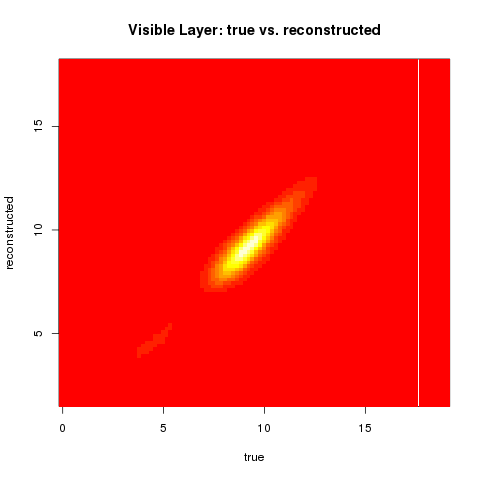
\includegraphics[width=0.3\columnwidth]{images/summer_school_2014-reconstruction-error-heatmap.pdf}~~\includegraphics[width=0.3\columnwidth]{images/summer_school_2014-reconstruction-error-boxplot.pdf}~~\includegraphics[width=0.3\columnwidth]{images/summer_school_2014-reconstruction-error-histogram.pdf}
\par\end{centering}
\caption[Rectionstruction error of data set breast\_cancer\_0.]{\label{fig:Reconstruction-error-breast_cancer_0}Rectionstruction
error of data set breast\_cancer\_0. Left: True (x-axis) versus reconstructed
(y-axis) expression values of data set breast\_cancer\_0. The heatmap
shows pixels from red over yellow to white. A pixel in red means zero
genes and the brighter a pixel is, the more genes there are in the
pixel's respective true and reconstructed expression value intervals.
Middle: Boxplot of reconstruction errors of the 10,000 most variable
genes. Right: Histogram of reconstruction errors of the 10,000 most
variable genes. Most genes have a low reconstruction error. Displayed
is the mean reconstruction error over all test samples.}
\end{figure}

Although the 10,000 numbers were compressed into only 50 numbers,
the mean reconstruction error of the 10,000 genes was only 0.563 (see
figure \ref{fig:Reconstruction-error-breast_cancer_0} middle). Considering
that the possible range (log2-intensities) of microarray values is
in the interval {[}0;16{]}, this is equivalent to a relative error
of 3.5\%. This demonstrated that RBMs are able to reduce dimensionality
of an expression data set while preserving most information.

\section{Prediction Quality From Labeled Samples\label{sec:breast_cancer_06-and-breast_cancer_07}}

\subsection{Increasing Number of Labeled Samples}

\index{breast_cancer_06@breast\_cancer\_06}The goal of data set breast\_cancer\_06
was to verify if basic training works. This was verified by testing
whether the classifier improves with an increasing amount of labeled
samples. Therefore we trained using all unlabeled samples, and defined
supervised learning data sets which have less and less labeled training
and test samples. Models were pre-trained using either an RBM or autoencoder
and fine-tuned with supervised back-propagation.

\paragraph{Definition of unlabeled data sets\label{par:Definition-of-unlabeled-data-sets-for-breast_cancer_06}}

A summary of unlabeled training, validation, and testing data sets
is shown in table \ref{tab:unlabeled-data-sets-of-breast_cancer_06}.
Validation samples were defined in case they were needed. Samples
from GSE17705 were included to give unsupervised training access to
more samples. (In later experiments, GSE17705 was left out to increase
the probability that samples are from the same distribution.)

\begin{table}
\begin{centering}
\begin{tabular}{|c|c|c||c|c||c||c|}
\hline 
 & GSE17705 & \multicolumn{2}{c|}{GSE25055} & \multicolumn{2}{c||}{GSE25065} & $\sum$\tabularnewline
\hline 
training & 239 & \multicolumn{2}{c|}{248} & \multicolumn{2}{c||}{159} & 646\tabularnewline
\hline 
validation & 29 & \multicolumn{2}{c|}{31} & \multicolumn{2}{c||}{19} & 79\tabularnewline
\hline 
testing & 30 & \multicolumn{2}{c|}{31} & \multicolumn{2}{c||}{20} & 81\tabularnewline
\hline 
\end{tabular}
\par\end{centering}
\caption{\label{tab:unlabeled-data-sets-of-breast_cancer_06}Sources of the
unlabeled data sets.}
\end{table}

\paragraph{Definition of labeled data sets}

To define the smaller and smaller labeled training data sets, we took
smaller and smaller fractions of the total 306 available labeled GSE25055
samples. The fractions were as displayed in table \ref{tab:training-and-validation-sets-of-breast_cancer_06}.

\noindent 
\begin{table}
\noindent \begin{centering}
\begin{tabular}{|c|c||c|c|c|c|c|c|c|}
\hline 
fraction & rep & \multicolumn{3}{c|}{training samples} & \multicolumn{3}{c|}{validation samples} & $\sum$\tabularnewline
\hline 
 &  & label 0 & label 1 & $\sum$ & label 0 & label 1 & $\sum$ & \tabularnewline
\hline 
\hline 
0.99 & 5 & 197 & 45 & 242 & 49 & 11 & 60 & 302\tabularnewline
\hline 
0.5 & 5 & 100 & 23 & 123 & 24 & 5 & 29 & 152\tabularnewline
\hline 
0.25 & 5 & 50 & 12 & 62 & 12 & 2 & 14 & 76\tabularnewline
\hline 
0.125 & 5 & 25 & 6 & 31 & 6 & 1 & 7 & 38\tabularnewline
\hline 
0.0625 & 5 & 12 & 3 & 15 & 3 & 0 & 3 & 18\tabularnewline
\hline 
\end{tabular}
\par\end{centering}
\caption[Sample distribution of training and validation sets of breast\_cancer\_06.]{\label{tab:training-and-validation-sets-of-breast_cancer_06}Sample
distribution of training and validation sets of data set breast\_cancer\_06.
The ``fraction'' in a data set denotes the fraction of the 306 labeled
samples GSE25055. The fraction of labeled samples used in a row is
split between training and validation data. Each of the 5 defined
data sets (rows) has 5 sub-sampled repetitions (``rep''), to be
able to draw error bars. Note that the number of samples is not balanced
between label 0 and label 1 samples.}
\end{table}

The testing set consists of all labeled GSE25065 samples, and no GSE25055
samples. (See table \ref{tab:Testing-set-for-breast_cancer_06}.)
Thus, betting on the largest group 0 yields an accuracy of $140/182\approx0.769$.

\noindent 
\begin{table}
\noindent \begin{centering}
\begin{tabular}{|c|c|c|c|c|c||c|}
\hline 
 & GSE17705 & \multicolumn{2}{c|}{GSE25055} & \multicolumn{2}{c||}{GSE25065} & \multirow{2}{*}{$\sum$}\tabularnewline
\cline{1-6} 
 &  & label 0 & label 1 & label 0 & label 1 & \tabularnewline
\hline 
\hline 
testing\_GSE25065 & 0 & 0 & 0 & 140 & 42 & 182\tabularnewline
\hline 
\end{tabular}
\par\end{centering}
\caption{\label{tab:Testing-set-for-breast_cancer_06}The testing set for data
set breast\_cancer\_06 consists of all labeled GSE25065 samples.}
\end{table}

In the next subsections, we describe the settings for pre-training
and fine-tuning.


\subsubsection{Unsupervised Pre-training Using RBM}

\index{breast_cancer_04_bg - bj@breast\_cancer\_04\_bg - bj}For unsupervised
pre-training of the RBM, we tried four different configurations that
are denoted in table \ref{tab:deepnet-settings-for-breast_cancer_04_bg-bj}.
(They were re-used from the runs labeled breast\_cancer\_04, which
are not described here.)

The reconstruction errors observed at the input layer during training
are shown in figure \ref{fig:reconstruction-errors-of-breast_cancer_04_bg-bj}.
In each training step, they (stochastically) decrease for all four
configurations and for training, validation, and testing data set.
Of note in this plot is that there is no overfitting since training
reconstruction error does not rise at the end of training. Also note
that the reconstruction error was not normalized to the number of
samples.

\begin{table}
\begin{centering}
\begin{tabular}{|c|c|c|c|c|}
\hline 
network instance & \_04\_bg & \_04\_bh & \_04\_bi & \_04\_bj\tabularnewline
\hline 
\hline 
network setting & value & value & value & value\tabularnewline
\hline 
\hline 
$base\textrm{\_}epsilon$ & 0.001 &  &  & \tabularnewline
\hline 
$activation$ & LOGISTIC &  &  & \tabularnewline
\hline 
$initial\textrm{\_}momentum$ & 0.5 &  &  & \tabularnewline
\hline 
$final\_momentum$ & 0.9 &  &  & \tabularnewline
\hline 
$momentum\textrm{\_}change\textrm{\_}steps$ & 3000 &  &  & \tabularnewline
\hline 
$sparsity$ & true &  &  & \tabularnewline
\hline 
$sparsity\textrm{\_}target$ & 0.5 & 0.5 & 0.25 & 0.1\tabularnewline
\hline 
$sparsity\textrm{\_}cost$ & 0.01 &  &  & \tabularnewline
\hline 
$sparsity\textrm{\_}damping$ & 0.9 &  &  & \tabularnewline
\hline 
$dropout$ & false &  &  & \tabularnewline
\hline 
$apply\textrm{\_}l2\textrm{\_}decay$ & true &  &  & \tabularnewline
\hline 
$l2\textrm{\_}decay$ & 0.001 &  &  & \tabularnewline
\hline 
\hline 
input layer setting & value & value & value & value\tabularnewline
\hline 
\hline 
$dimensions$ & 500 &  &  & \tabularnewline
\hline 
$sparsity$ & false &  &  & \tabularnewline
\hline 
\hline 
hidden layer 1 setting & value & value & value & value\tabularnewline
\hline 
\hline 
$dimensions$ & 500 & 1000 & 1000 & 1000\tabularnewline
\hline 
\end{tabular}
\par\end{centering}
\caption[\emph{deepnet }settings for unsupervised pre-training RBMs breast\_cancer\_04\_bg
- bj.]{\label{tab:deepnet-settings-for-breast_cancer_04_bg-bj}\emph{deepnet
}settings for unsupervised pre-training RBMs breast\_cancer\_04\_bg
- bj. No entry in a cell means that it has the same value as the cell
to the left.}
\end{table}

\begin{figure}
\begin{centering}
\includegraphics[width=0.35\columnwidth]{images/breast_cancer_04-plot-bg_bj}
\par\end{centering}
\caption[Reconstruction error of training, validation and testing data sets.]{\label{fig:reconstruction-errors-of-breast_cancer_04_bg-bj}Reconstruction
errors of training (T\_E), validation (V\_E) and testing (E\_E) data
sets for unsupervised training of an RBM with configurations breast\_cancer\_04\_bg,
bh, bi, bj. The y-axis is the reconstruction error, not normalized
for the number of samples, and the x-axis is the training step of
neural network training.}
\end{figure}

\subsubsection{Supervised Classification with Unsupervisedly Pre-trained RBM}

The settings for the supervised training runs \index{breast_cancer_06_aa - ad@breast\_cancer\_06\_aa - ad}breast\_cancer\_06\_aa
- ad were as described in table \ref{tab:deepnet-settings-for-breast_cancer_06_aa-ad}.
Four different models were tested, differing in number of nodes in
hidden layer 1 (setting $dimensions$) and the pre-trained weights
and biases between the input layer and hidden layer 1 (setting $pretrained\textrm{\_}model$).

\begin{table}
\begin{centering}
\begin{tabular}{|c|c|c|c|c|}
\hline 
network instance & \_06\_aa & \_06\_ab & \_06\_ac & \_06\_ad\tabularnewline
\hline 
\hline 
network setting & value & value & value & value\tabularnewline
\hline 
\hline 
$base\textrm{\_}epsilon$ & 0.001 &  &  & \tabularnewline
\hline 
$activation$ & LOGISTIC &  &  & \tabularnewline
\hline 
$initial\textrm{\_}momentum$ & 0.5 &  &  & \tabularnewline
\hline 
$final\_momentum$ & 0.9 &  &  & \tabularnewline
\hline 
$momentum\textrm{\_}change\textrm{\_}steps$ & 3000 &  &  & \tabularnewline
\hline 
$dropout$ & true &  &  & \tabularnewline
\hline 
$dropout\textrm{\_}prob$ & 0.5 &  &  & \tabularnewline
\hline 
$apply\textrm{\_}l2\textrm{\_}decay$ & true &  &  & \tabularnewline
\hline 
$l2\textrm{\_}decay$ & 0.001 &  &  & \tabularnewline
\hline 
\hline 
input layer setting & value & value & value & value\tabularnewline
\hline 
\hline 
$dimensions$ & 500 &  &  & \tabularnewline
\hline 
$dropout\textrm{\_}prob$ & 0.2 &  &  & \tabularnewline
\hline 
\hline 
hidden layer 1 setting & value & value & value & value\tabularnewline
\hline 
\hline 
$dimensions$ & 500 & 1000 & 1000 & 1000\tabularnewline
\hline 
$pretrained\textrm{\_}model$ & \_04\_bg & \_04\_bh & \_04\_bi & \_04\_bj\tabularnewline
\hline 
\hline 
output layer setting & value & value & value & value\tabularnewline
\hline 
\hline 
$dimensions$ & 1 &  &  & \tabularnewline
\hline 
$loss\textrm{\_}function$ & CROSS\_ENTROPY &  &  & \tabularnewline
\hline 
$activation$ & SOFTMAX &  &  & \tabularnewline
\hline 
$dropout$ & false &  &  & \tabularnewline
\hline 
\end{tabular}
\par\end{centering}
\caption[$deepnet$ settings for the classifiers breast\_cancer\_06\_aa - ad.]{\label{tab:deepnet-settings-for-breast_cancer_06_aa-ad}$deepnet$
settings for the classifiers breast\_cancer\_06\_aa - ad. Each classifier
is initialized using an unsupervisedly pre-trained RBM, and trained
supervisedly on data set breast\_cancer\_06. No entry in a cell means
that it has the same value as the cell to the left. The only difference
between the four configurations is the hidden layer 1 size ($dimensions$)
and initialization ($pretrained\textrm{\_}model$).}
\end{table}

For each of the $5$ differently sized training data sets, for each
of the $5$ repetitions, and for each of the $4$ differently pre-trained
RBMs, a classifier was trained. (So altogether $5*5*4=100$ classifiers
were trained.) Performance was then assessed through the accuracy,
as shown in figure \ref{fig:accuracy-plots-of-breast_cancer_06_aa-ad}.

\begin{figure}
\begin{centering}
\includegraphics[width=0.68\paperwidth]{images/breast_cancer_06-loess-aa_ad.pdf}
\par\end{centering}
\caption[Box plots showing the accuracies of the models breast\_cancer\_06\_aa
- ad.]{\label{fig:accuracy-plots-of-breast_cancer_06_aa-ad}Box plots showing
the accuracies of the models breast\_cancer\_06\_aa - ad. Each panel
shows one of the four configurations breast\_cancer\_06\_aa - ad.
In each panel, the x-axis shows the number of labeled samples in the
5 different data sets. The y-axis shows the smoothed accuracy, as
described in section \ref{subsec:Model-selection}. Each dot is the
accuracy of a repetition in the respective data set.}
\end{figure}

Surprisingly, the neural network accuracies do not improve with increasing
number of labeled samples. Instead it seems that the classifiers using
the least and most (18 and 302) samples perform best, and all others
(especially those using 76 samples) perform worst. As we will see,
this is due to an unbalanced number of label 0 and label 1 samples
in the training set. The tendency that the accuracies for 18 labeled
samples are about as high as those for 302 labeled samples, and are
the lower the closer the number of labeled samples are to 76 samples,
could be due to using the same pre-trained hidden-layer weights and
biases across the 5 repetitions. (The supervised training and validation
data are sampled independelty though.)

We also tried using 2 hidden layers instead of 1. This did not improve
accuracy.

\subsubsection{Unsupervised Pre-training Using Autoencoder\label{subsec:Unsupervised-pre-training-using-autoencoder}}

\index{breast_cancer_03_ai@breast\_cancer\_03\_ai}\index{breast_cancer_03_al@breast\_cancer\_03\_al}\index{breast_cancer_03_am@breast\_cancer\_03\_am}\index{breast_cancer_03_ao@breast\_cancer\_03\_ao}Settings
for unsupervised pre-training of the autoencoders are given in table
\ref{tab:deepnet-settings-for-breast_cancer_03_ai,_al,_am,_ao} (named
breast\_cancer\_03\_ai - am,ao). The only differences between the
models are in $base\mbox{\_}epsilon$ and $activation$.

\begin{table}
\begin{centering}
\begin{tabular}{|c|c|c|c|c|}
\hline 
network instance & \_03\_ai & \_03\_al & \_03\_am & \_03\_ao\tabularnewline
\hline 
\hline 
network setting & value & value & value & value\tabularnewline
\hline 
\hline 
$base\textrm{\_}epsilon$ & 1.0 & 0.01 & 0.01 & 0.1\tabularnewline
\hline 
$activation$ & LOGISTIC & RECTIFIED\_LINEAR & LOGISTIC & \tabularnewline
\hline 
$initial\textrm{\_}momentum$ & 0.5 &  &  & \tabularnewline
\hline 
$final\_momentum$ & 0.99 &  &  & \tabularnewline
\hline 
$momentum\textrm{\_}change\textrm{\_}steps$ & 50000 &  &  & \tabularnewline
\hline 
$dropout$ & true &  &  & \tabularnewline
\hline 
$dropout\textrm{\_}prob$ & 0.5 &  &  & \tabularnewline
\hline 
$apply\textrm{\_}l2\textrm{\_}decay$ & false &  &  & \tabularnewline
\hline 
$l2\textrm{\_}decay$ & 0.0001 &  &  & \tabularnewline
\hline 
\hline 
input layer setting & value & value & value & value\tabularnewline
\hline 
\hline 
$dimensions$ & 500 &  &  & \tabularnewline
\hline 
$dropout\textrm{\_}prob$ & 0.2 &  &  & \tabularnewline
\hline 
\hline 
hidden layer 1 setting & value & value & value & value\tabularnewline
\hline 
\hline 
$dimensions$ & 1000 &  &  & \tabularnewline
\hline 
\end{tabular}
\par\end{centering}
\caption[Settings for the unsupervised pre-training autoencoders breast\_cancer\_03\_ai,
\_03\_al, \_03\_am, and \_03\_ao.]{\label{tab:deepnet-settings-for-breast_cancer_03_ai,_al,_am,_ao}Settings
for the unsupervised pre-training autoencoders breast\_cancer\_03\_ai,
\_03\_al, \_03\_am, and \_03\_ao. No entry in a cell means that it
has the same value as the cell to the left.}
\end{table}

\subsubsection{Supervised Classification with Unsupervisedly Pre-trained Autoencoder}

\index{breast_cancer_06_ae - ah@breast\_cancer\_06\_ae - ah}When
training a neural network using back-propagation that was pre-trained
using one of the four autoencoders described in the previous section,
the resulting accuracy plots looked similar to the ones when pre-training
with an RBM (plots not shown). As we will see, similar to pre-training
using RBMs, this is due to an uneven number of label 0 and label 1
samples in the training set.

Like for RBMs, we also tried using 2 hidden layers instead of 1, but
this did not improve accuracy.

\subsubsection{High Label Prediction Bias\label{par:Examining-biased-classifier}}

\index{breast_cancer_06_aa/_n302_cv1@breast\_cancer\_06\_aa/\_n302\_cv1}The
lack of the accuracy increasing with the number of labeled training
samples can be explained by the following observation.

When examining the predictions of model breast\_cancer\_06\_aa/\_n302\_cv1
(the first network pre-trained on 302 samples), it becomes evident
that the training is sub-optimal, because label 0 is predicted almost
exclusively.  Table \ref{tab:predictions-of-breast_cancer_06_aa/_n302_cv1}
shows the predicted classes. 
\begin{table}
\begin{centering}
\begin{tabular}{|c|c|c|}
\hline 
 & label 0 & label 1\tabularnewline
\hline 
\hline 
training & 240 & 2\tabularnewline
\hline 
validation & 58 & 2\tabularnewline
\hline 
testing & 182 & 0\tabularnewline
\hline 
\end{tabular}
\par\end{centering}
\caption{\label{tab:predictions-of-breast_cancer_06_aa/_n302_cv1}Predictions
of the network breast\_cancer\_06\_aa/\_n302\_cv1.}
\end{table}

There is a heavy bias in favor of label 0. Our hypothesis was that
this is due to the unbalanced class label distribution in data set
breast\_cancer\_06. Therefore, the next data set is balanced in this
regard.

\subsection{Equal Number of Class Labels \label{subsec:Increasing-number-of-labeled-samples-and-equal-number-of-class-labels}}

As in the previous section on breast\_cancer\_06, in data set \index{breast_cancer_07@breast\_cancer\_07}breast\_cancer\_07,
we wanted to check whether the artificial neural networks accuracies
improve with an increasing number of labeled samples. Unlabeled data
sets were the same as for breast\_cancer\_06, see table \vref{tab:unlabeled-data-sets-of-breast_cancer_06}.
In contrast to the previous data set breast\_cancer\_06, each labeled
data set contains as many label 0 samples as label 1 samples (see
table \ref{tab:Data-set-breast_cancer_07}). The testing data set
is the same as in breast\_cancer\_06 and exclusively consists of GSE25065
samples, see table \vref{tab:Testing-set-for-breast_cancer_06}.

\begin{table}
\noindent \begin{centering}
\begin{tabular}{|c|c|c|c|c|c|c|c|c|}
\hline 
\multirow{2}{*}{data set} & \multirow{2}{*}{rep} & \multicolumn{3}{c|}{training samples} & \multicolumn{3}{c|}{validation samples} & \multirow{2}{*}{$\sum$}\tabularnewline
\cline{3-8} 
 &  & label 0 & label 1 & $\sum$ & label 0 & label 1 & $\sum$ & \tabularnewline
\hline 
\hline 
1 & 5 & 45 & 45 & 90 & 49 & 11 & 60 & 150\tabularnewline
\hline 
2 & 5 & 23 & 23 & 46 & 24 & 5 & 29 & 75\tabularnewline
\hline 
3 & 5 & 12 & 12 & 24 & 12 & 2 & 14 & 38\tabularnewline
\hline 
4 & 5 & 6 & 6 & 12 & 6 & 1 & 7 & 19\tabularnewline
\hline 
5 & 5 & 3 & 3 & 6 & 3 & 0 & 3 & 9\tabularnewline
\hline 
\end{tabular}
\par\end{centering}
\caption[Samples in data set breast\_cancer\_07.]{\label{tab:Data-set-breast_cancer_07}Samples in data set breast\_cancer\_07.
``rep'' is the number of subsamplings from all samples described
by a line in the table. Note that there is an equal number of training
samples for each class, but an unequal number in the validation data
sets.}
\end{table}

Only the 500 most variable genes were used. The training and validation
data sets were generated from subsets of GSE25055. Each training data
set had an equal number of samples from class 0 and class 1. However,
the validation data sets contained a larger number of class 0 samples,
because there were only 57 label 1 samples in GSE25055, and 45 of
them were needed for training. The test data set is composed of all
GSE25065 samples. Each data set was drawn 5 times from the samples
as described for training and validation data set. This is to repeat
the experiment 5 times and to be able to obtain error bars for the
accuracies.

If we were to bet on the larger test set class we would achieve an
accuracy of $140/182=0.769$, because the test set contains 140 label
0 samples, but only 42 label 1 samples. However, because the training
data set contains an equal number of label 0 and label 1 samples,
the test set accuracy should not be as biased as data set breast\_cancer\_06,
whose training data set is imbalanced.

The following machine learning algorithms were tested on this data
set: SVM, TSVM, supervised classification with unsupervised pre-trained
RBM, supervised classification with unsupervisedly pre-trained autoencoder,
supervised classification without pre-training. Unsupervised pre-training
was performed as for breast\_cancer\_06.

\subsubsection{SVM Accuracies}

\begin{figure}
\begin{centering}
\includegraphics[width=0.34\paperwidth]{images/breast_cancer_07-accuracies-svm-testing.pdf}
\par\end{centering}
\caption[Accuracy box plots of SVM predicting data set breast\_cancer\_07.]{\label{fig:Accuracy-box-plots-of-SVM-on-breast_cancer_07}Accuracy
box plots of SVM predicting the testing data of breast\_cancer\_07.
On the x-axis are the sizes of the data sets containing an increasing
number of labeled samples. On the y-axis are the accuracies obtained
on the testing data.}
\end{figure}

Figure \ref{fig:Accuracy-box-plots-of-SVM-on-breast_cancer_07} shows
there is the tendency that adding more samples to supervised learning
yields better accuracy. Although the 25\%- and 75\%-quantile of the
boxplots suggest different variances, we believe that the boxplots
should not be over-interpreted, as there are only 5 data points (5
subsamplings).

\subsubsection{TSVM Accuracies}

TSVM can utilize incomplete and unlabelled data to improve supervised
classification (``transductive SVM''). Figure \ref{fig:Accuracy-box-plots-of-TSVM-on-breast_cancer_07}
shows that TSVM sometimes fails to learn a model for the data sets
with less than 46 labeled samples and otherwise performs similarly
to a normal SVM.

\begin{figure}
\begin{centering}
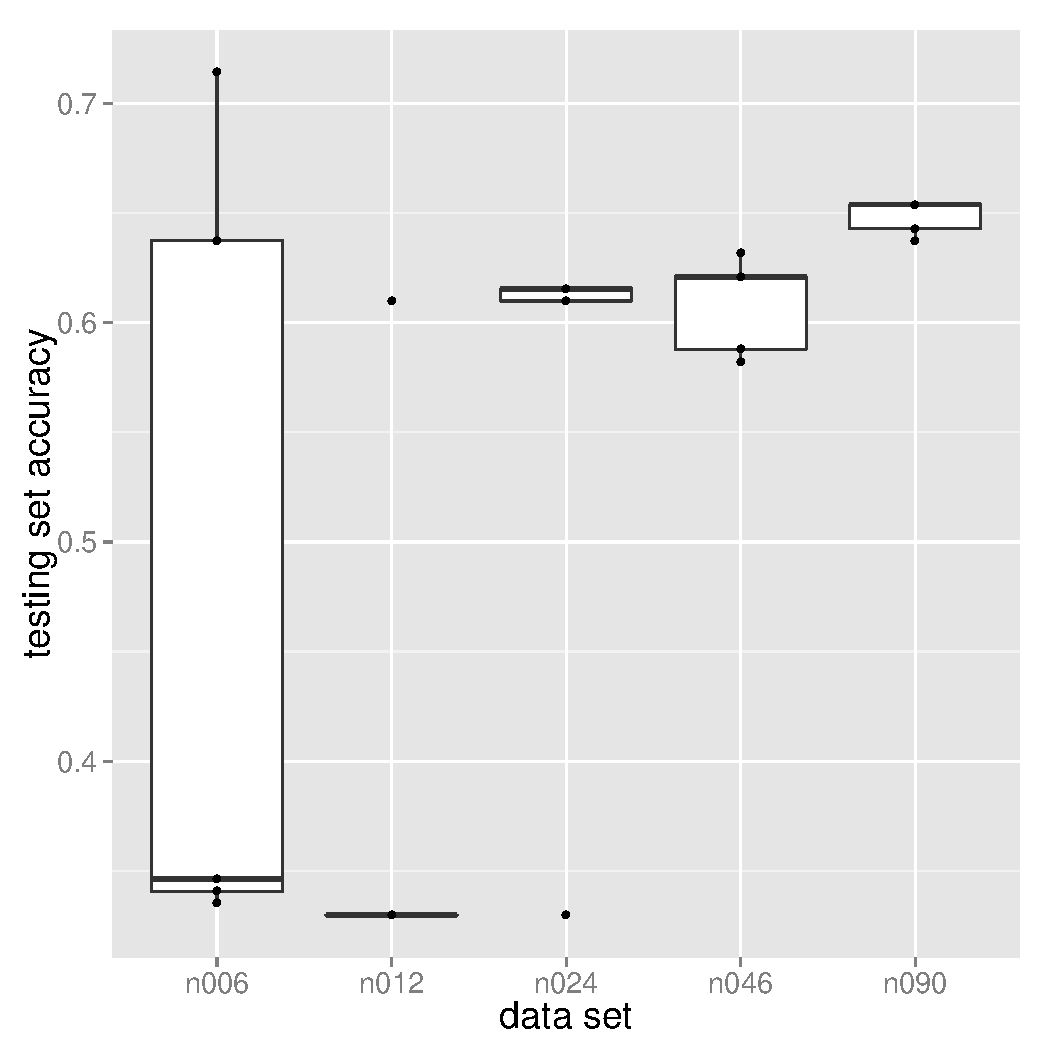
\includegraphics[width=0.34\paperwidth]{images/breast_cancer_07-accuracies-svmlight.pdf}
\par\end{centering}
\caption[Accuracy box plots of TSVM predicting data set of breast\_cancer\_07.]{\label{fig:Accuracy-box-plots-of-TSVM-on-breast_cancer_07}Accuracy
box plots of TSVM predicting the testing data set of breast\_cancer\_07.
On the x-axis are the sizes of the data sets containing an increasing
number of labeled samples. On the y-axis are the accuracies obtained
on the testing data.}
\end{figure}

\subsubsection{Supervised Classification with Unsupervisedly Pre-trained RBM}

The \emph{deepnet }settings for training runs \index{breast_cancer_07_aa - ad@breast\_cancer\_07\_aa - ad}breast\_cancer\_07\_aa
- ad were the same as those for breast\_cancer\_06\_aa - ad (see table
\vref{tab:deepnet-settings-for-breast_cancer_06_aa-ad}).

As expected, the accuracy plots in figure \ref{fig:Accuracy-box-plots-of-breast_cancer_07_aa-ad}
show that all 4 neural networks perform better the more labeled samples
there are in training. In addition the variance of the accuracies
decreases, the more labeled samples there are in training.

\begin{figure}
\begin{centering}
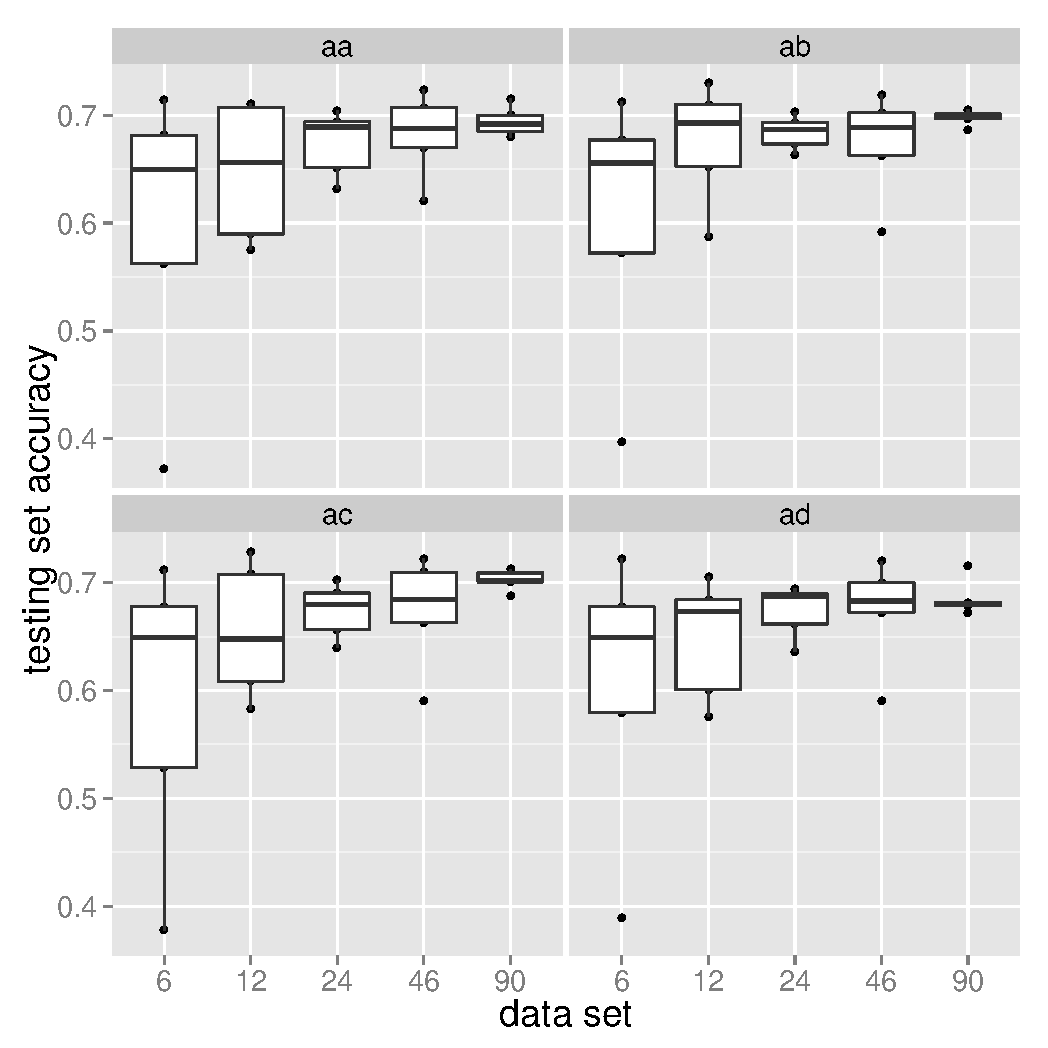
\includegraphics[width=0.68\paperwidth]{images/breast_cancer_07-accuracies-aa_ad.pdf}
\par\end{centering}
\caption[Accuracy box plots of a feed-forward neural network pre-trained with
an RBM, predicting the testing data set of breast\_cancer\_07.]{\label{fig:Accuracy-box-plots-of-breast_cancer_07_aa-ad}Accuracy
box plots of a feed-forward neural network pre-trained with an RBM,
predicting the testing data set of breast\_cancer\_07. On the x-axis
are the sizes of the data sets containing an increasing number of
labeled samples. On the y-axis are the accuracies obtained on the
testing data.}
\end{figure}

\subsubsection{Supervised Classification with Unsupervisedly Pre-trained Autoencoder}

The settings for \emph{deepnet }training of \index{breast_cancer_07_ae - ah@breast\_cancer\_07\_ae - ah}breast\_cancer\_07\_ae
- ah were as those for breast\_cancer\_06\_ae - ah. As is shown in
figure \ref{fig:Accuracy-box-plots-of-breast_cancer_07_ae-ah}, pre-training
with an autoencoder yields similar accuracies as pre-training with
an RBM.

\begin{figure}
\begin{centering}
\includegraphics[width=0.68\paperwidth]{images/breast_cancer_07-accuracies-ae_ah.pdf}
\par\end{centering}
\caption[Accuracy box plots of a feed-forward neural network pre-trained with
an autoencoder, predicting the testing data set of breast\_cancer\_07.]{\label{fig:Accuracy-box-plots-of-breast_cancer_07_ae-ah}Accuracy
box plots of a feed-forward neural network pre-trained with an autoencoder,
predicting the testing data set of breast\_cancer\_07. On the x-axis
are the sizes of the data sets containing an increasing number of
labeled samples. On the y-axis are the accuracies obtained on the
testing data.}
\end{figure}

\subsubsection{Supervised Classification without Pre-training}

Finally, in \index{breast_cancer_07_ai - aj@breast\_cancer\_07\_ai - aj}breast\_cancer\_07\_ai
- aj, we trained the neural networks with no pre-training at all,
but using only back-propagation. The \emph{deepnet} settings are shown
in table \ref{tab:deepnet-settings-for-breast_cancer_07_ai-aj}.

\begin{table}
\begin{centering}
\begin{tabular}{|c|c|c|}
\hline 
network instance & \_07\_ai & \_07\_aj\tabularnewline
\hline 
\hline 
network setting & value & value\tabularnewline
\hline 
\hline 
$base\textrm{\_}epsilon$ & 0.001 & \tabularnewline
\hline 
$activation$ & LOGISTIC & \tabularnewline
\hline 
$initial\textrm{\_}momentum$ & 0.5 & \tabularnewline
\hline 
$final\_momentum$ & 0.9 & \tabularnewline
\hline 
$momentum\textrm{\_}change\textrm{\_}steps$ & 3000 & \tabularnewline
\hline 
$dropout$ & true & false\tabularnewline
\hline 
$dropout\textrm{\_}prob$ & 0.5 & \tabularnewline
\hline 
$apply\textrm{\_}l2\textrm{\_}decay$ & true & \tabularnewline
\hline 
$l2\textrm{\_}decay$ & 0.001 & \tabularnewline
\hline 
\hline 
input layer setting & value & value\tabularnewline
\hline 
\hline 
$dimensions$ & 500 & \tabularnewline
\hline 
$dropout\textrm{\_}prob$ & 0.2 & \tabularnewline
\hline 
\hline 
hidden layer 1 setting & value & value\tabularnewline
\hline 
\hline 
$dimensions$ & 1000 & \tabularnewline
\hline 
$initialization$ & CONSTANT & \tabularnewline
\hline 
\hline 
output layer setting & value & value\tabularnewline
\hline 
\hline 
$dimensions$ & 1 & \tabularnewline
\hline 
$loss\textrm{\_}function$ & CROSS\_ENTROPY & \tabularnewline
\hline 
$activation$ & SOFTMAX & \tabularnewline
\hline 
$dropout$ & false & \tabularnewline
\hline 
\end{tabular}
\par\end{centering}
\caption[Settings for the classifiers breast\_cancer\_07\_ai - aj.]{\label{tab:deepnet-settings-for-breast_cancer_07_ai-aj}Settings
for the classifiers breast\_cancer\_07\_ai - aj, which is trained
using backpropagation only (without pre-training). Each classifier
is trained supervisedly on data set breast\_cancer\_07. The only difference
between the two configurations is the use of $dropout$ in breast\_cancer\_07\_ai.
No entry in a cell means that it has the same value as the cell to
the left.}
\end{table}

\begin{figure}
\begin{centering}
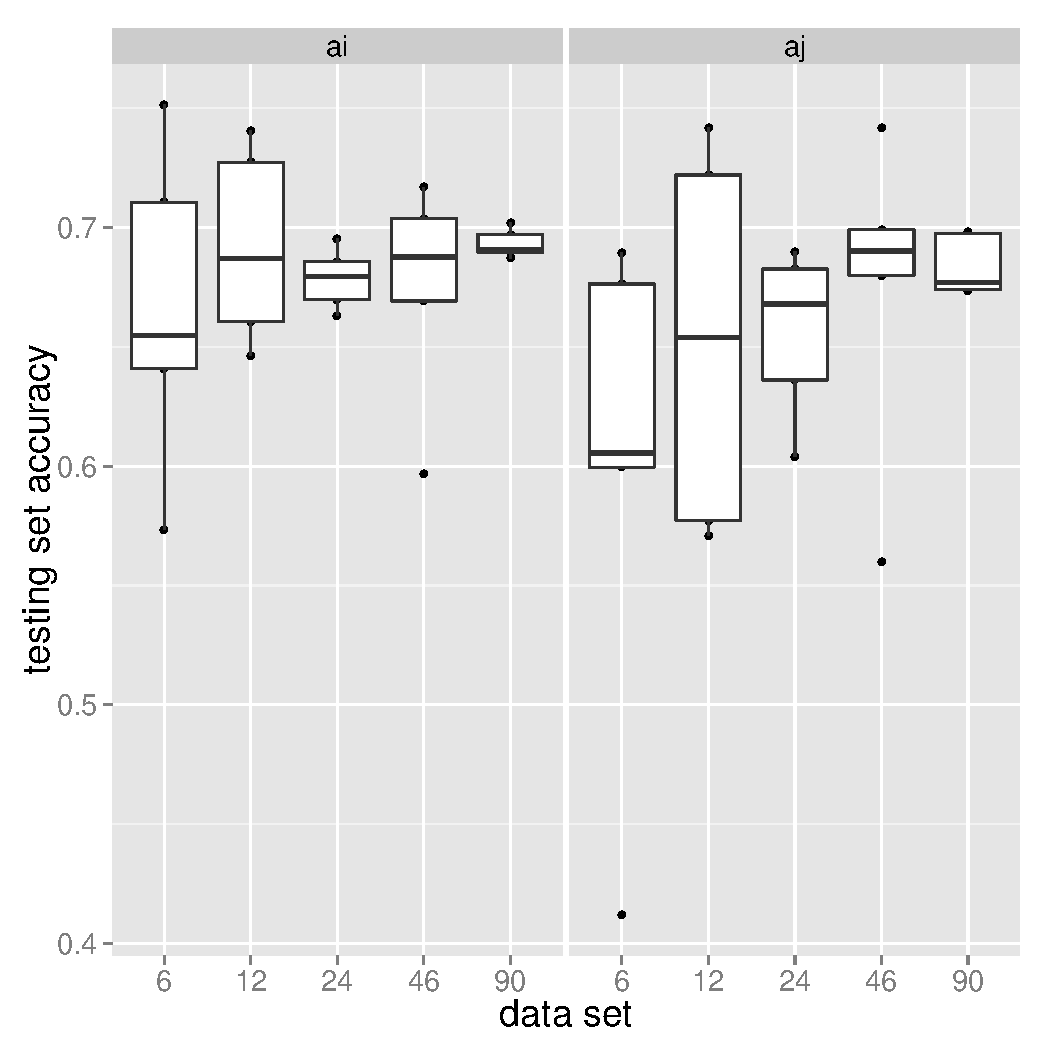
\includegraphics[width=0.68\paperwidth]{images/breast_cancer_07-accuracies-ai_aj.pdf}
\par\end{centering}
\caption[Accuracy box plots of feed-forward neural networks not pre-trained,
predicting the testing data set of breast\_cancer\_07.]{\label{fig:Accuracy-box-plots-of-breast_cancer_07_ai-aj}Accuracy
box plots of feed-forward neural networks not pre-trained, predicting
the testing data set of breast\_cancer\_07. On the x-axis are the
sizes of the data sets containing an increasing number of labeled
samples. On the y-axis are the accuracies obtained on the testing
data. The panel ``ai'' stands for the classifier ``breast\_cancer\_07\_ai'',
``aj'' for ``breast\_cancer\_07\_aj''.}
\end{figure}

The accuracy plots are shown in figure \ref{fig:Accuracy-box-plots-of-breast_cancer_07_ai-aj}.
As can be seen, using $dropout$ (breast\_cancer\_07\_ai) yields better
accuracies than not using it (breast\_cancer\_07\_aj). An explanation
can be that \emph{$dropout$} reduces overfitting. In addition, comparing
with the neural networks pre-trained using RBM or autoencoder (e.g.
breast\_cancer\_07\_ai versus breast\_cancer\_07\_ag) might indicate
a slight advantage of not using pre-training (but using $dropout$)
in the data sets with little labeled samples. However, this assertion
should be re-done with more than 5 repetitions.

The accuracies of the classifiers on breast\_cancer\_07 are lower
than those on breast\_cancer\_06. This indicates the higher difficulty
of the classification task when the labels are balanced. We will look
into this in the following.

\subsubsection{Confusion Table of Predicted Classes}

Like for breast\_cancer\_06, we looked at the output of one of the
neuronal networks trained on data set breast\_cancer\_07. As can be
seen in table \ref{tab:predictions-of-breast_cancer_07_aa} and in
contrast to the predictions on data set breast\_cancer\_06, the predicted
classes are now more balanced.

\begin{table}
\begin{centering}
\begin{tabular}{|c|c|c|}
\hline 
 & label 0 & label 1\tabularnewline
\hline 
\hline 
training & 44 & 46\tabularnewline
\hline 
validation & 38 & 22\tabularnewline
\hline 
testing & 117 & 65\tabularnewline
\hline 
\end{tabular}
\par\end{centering}
\caption{\label{tab:predictions-of-breast_cancer_07_aa}Labels predicted by
\index{breast_cancer_07_aa/_n090_cv1@breast\_cancer\_07\_aa/\_n090\_cv1}breast\_cancer\_07\_aa/\_n090\_cv1
on training, validation, and testing data set.}
\end{table}

\paragraph{Confusion table on the test set samples}

\begin{table}
\begin{centering}
\begin{tabular}{|c||c|c|}
\hline 
 & true label 0 & true label 1\tabularnewline
\hline 
\hline 
predicted label 0 & 101 & 16\tabularnewline
\hline 
predicted label 1 & 39 & 26\tabularnewline
\hline 
\end{tabular}
\par\end{centering}
\caption[Confusion table of the predictions made by breast\_cancer\_07\_aa/\_n090.]{\label{tab:Confusion-table-of-breast_cancer_07_aa/_n090_cv1}Confusion
table of the predictions made by breast\_cancer\_07\_aa/\_n090\_cv1
(which was trained on 90 labeled samples) on the testing data set
of data set breast\_cancer\_07.}
\end{table}

The confusion table \ref{tab:Confusion-table-of-breast_cancer_07_aa/_n090_cv1}
shows the predicted and true labels in the testing data set. It shows
that most predicted label 1 samples are actually label 0 samples ($\frac{39}{39+26}$).
Of the true label 0 samples, $\frac{101}{101+39}\approx0.72$ are
classified correctly, and $\frac{26}{26+16}\approx0.62$ of the true
label 1 samples. This may indicate that predicting label 1 samples,
which means ``pathologic complete response'', i.e. no remaining
breast cancer, is more difficult than predicting ``residual disease''.

The predicted probabilities of the true class of the mis-classified
samples (i.e. those not on the main diagonal) can be displayed in
a histogram, see figure \ref{fig:Histogram-of-probabilities-of-breast_cancer_07}.
The histogram shows that the probabilities for the true class of mis-classified
samples are not mostly near 0.5, but in the middle of the possible
range. 0.5 is the maximum probability, otherwise the sample would
not be mis-classified.

\begin{figure}
\begin{centering}
\includegraphics[width=0.68\columnwidth]{images/breast_cancer_07-true-label-probabilities-of-misclassified-samples.pdf}
\par\end{centering}
\caption[Histogram of probabilities of samples predicted wrongly.]{\label{fig:Histogram-of-probabilities-of-breast_cancer_07}Histogram
of probabilities of samples predicted wrongly by breast\_cancer\_07\_aa/\_n090\_cv1.
The x-axis is the predicted probability of the true class; the y-axis
the counts of samples.}
\end{figure}

\section{Different Normalizations\label{sec:breast_cancer_08}}

One of the goals of this work was to show that adding unlabeled samples
increases accuracy in semi-supervised classification. To achieve that
goal, in \index{breast_cancer_08@breast\_cancer\_08}breast\_cancer\_08,
we built data sets with a constant number of labeled samples and an
increasing number of unlabeled samples.

To alleviate the effects of systematic errors in the raw data, we
tried different normalizations in order to search for normalizations
that are beneficial to classification accuracy. We assessed the effect
of different normalizations on unsupervised pre-training using an
autoencoder and supervised classification accuracy.

\subsection{Data Set Design}

Table \ref{tab:design-of-breast_cancer_08} shows the assignment of
samples to data sets. Note that labeled training and validation data
are almost exclusively from GSE25055, and labeled testing data are
exclusively from GSE25065.

Labeled training and testing data are balanced with respect to the
number of label 0 and label 1 samples. An unbalanced data set leads
to a biased classifier which prefers the label it was shown more often
during training. (As was demonstrated on page \pageref{par:Examining-biased-classifier}.)
The increasing number of unlabeled training data are mostly from GSE25055,
except data set 4, which also has unlabeled data from GSE25065. The
unlabeled training data are balanced in data sets 1 and 2, and in
proportions 1:2 and 1:4 in data sets 3 and 4, respectively.

\begin{table}
\begin{centering}
\begin{tabular}{|c|c||c|c|c|c|}
\hline 
 & data source & data set 1 & data set 2 & data set 3 & data set 4\tabularnewline
\hline 
\hline 
labeled training & GSE25055 & 28\textbar{}28 & 28\textbar{}28 & 28\textbar{}28 & 28\textbar{}28\tabularnewline
\hline 
\multirow{2}{*}{unlabeled training} & GSE25055 & 15\textbar{}15 & 29\textbar{}29 & 58\textbar{}29 & 58\textbar{}29\tabularnewline
\cline{2-6} 
 & GSE25065 & 0\textbar{}0 & 0\textbar{}0 & 0\textbar{}0 & 58\textbar{}0\tabularnewline
\hline 
\multirow{2}{*}{labeled validation} & GSE25055 & 221\textbar{}29 & 221\textbar{}29 & 221\textbar{}29 & 221\textbar{}29\tabularnewline
\cline{2-6} 
 & GSE25065 & 0\textbar{}0 & 0\textbar{}0 & 0\textbar{}0 & 0\textbar{}0\tabularnewline
\hline 
labeled testing & GSE25065 & 42\textbar{}42 & 42\textbar{}42 & 42\textbar{}42 & 42\textbar{}42\tabularnewline
\hline 
repeats &  & 5 & 5 & 5 & 5\tabularnewline
\hline 
proportions 0:1 &  & 1:1 & 1:1 & 2:1 & 4:1\tabularnewline
\hline 
\end{tabular}
\par\end{centering}
\caption[The design of data set breast\_cancer\_08.]{\label{tab:design-of-breast_cancer_08}The design of data set breast\_cancer\_08.
There are 4 sub-data-sets that have a constant number of labeled training,
labeled validation, and labeled testing samples. The unlabeled data
sets have an increasing number of samples. The syntax ``$x$\textbar{}$y$''
in a table cell means that there are $x$ samples having label 0,
and $y$ samples having label 1. The row ``repeats'' means that
each data set was created 5 times, by random sampling. The row ``proportions
0:1'' describes the relative proportions of label 0 and label 1 samples
in the ``unlabeled training'' rows.}
\end{table}

\pagebreak{}

\subsection{Normalizations}

We used RMA \cite{BolstadSpeed2003}, MAS5 \cite{Affymetrix2001},
MAS5+log2, RMA+ComBat, MAS5+ComBat, and MAS5+log2+ComBat to normalize
the raw microarray data (for ComBat, see \cite{JohnsonRabinovic2007}).
Because MAS5 does not logarithmize the data, but RMA does, MAS5 was
tried with additional logarithmizing of the data. ComBat was designed
as a batch-effect correction method. It produces a data set with the
same size as the original one, but with batch-effects between samples
removed. As input, ComBat needs the expression matrix and, for each
sample, the batch. We defined samples from the two sources GSE25055
and GSE25065 as batches. Table \ref{tab:normalizations-for-breast_cancer_08}
shows a list of different normalizations.

\begin{table}
\begin{centering}
\begin{tabular}{|c|c|c|}
\hline 
configuration & normalization & normalizations applied\tabularnewline
\hline 
\hline 
breast\_cancer\_08\_bb - bx & rma & RMA\tabularnewline
\hline 
breast\_cancer\_08\_by - cu & mas5 & MAS5\tabularnewline
\hline 
breast\_cancer\_08\_ep - fl & rma,combat & RMA, ComBat batch effect correction\tabularnewline
\hline 
breast\_cancer\_08\_fm - gi & mas5,combat & MAS5, ComBat batch effect correction\tabularnewline
\hline 
\end{tabular}
\par\end{centering}
\caption{\label{tab:normalizations-for-breast_cancer_08}Data set normalizations
tested in breast\_cancer\_08.}
\end{table}

For each of 4 different normalization pre-processing combinations,
we created each of the 4 data sets by random sampling from the designated
samples described in table \ref{tab:design-of-breast_cancer_08}.
The normalization steps were done in this order: first RMA/MAS5 normalization
and summarization (to default HG\_U133A probe sets), then ComBat (if
enabled), then splitting of the data matrices into the sub-data-sets
according to table \ref{tab:design-of-breast_cancer_08}.

\begin{table}
\begin{centering}
\begin{tabular}{|c||c|c|c|c|}
\hline 
\multirow{2}{*}{normalization} & \multicolumn{4}{c|}{data set}\tabularnewline
\cline{2-5} 
 & 1 & 2 & 3 & 4\tabularnewline
\hline 
\hline 
rma & 0.23 (.0032) & 0.41 (.0075) & 0.61 (.0061) & 1.02 (.016)\tabularnewline
\hline 
mas5 & 0.045 (.0022) & 0.053 (.00041) & 0.058 (.002) & 0.068 (.0029)\tabularnewline
\hline 
rma,combat & 0.24 (.0038) & 0.4 (.0028) & 0.6 (.0052) & 1.02 (.016)\tabularnewline
\hline 
mas5,combat & 0.057 (.0035) & 0.07 (.0011) & 0.079 (.0033) & 0.088 (.0034)\tabularnewline
\hline 
\end{tabular}
\par\end{centering}
\caption[Reconstruction error for differently normalized data.]{\label{tab:Reconstruction-error-for-breast_cancer_08}Reconstruction
error for differently normalized data. In the rows are the different
normalizations, and in the columns the data sets. Each cell in the
table contains the mean (and standard deviation in brackets) of the
reconstruction error over all repeats. The numbers are rounded to
two significant digits. Reconstruction errors shown for MAS5 were
computed on not logarithmized data.}
\end{table}

\subsection{Unsupervised Reconstruction Error in Autoencoder Pre-training}

Before looking at the accuracies of the supervised classifier, we
looked at unsupervised pre-training using an autoencoder. The reconstruction
error for each normalization is shown in table \ref{tab:Reconstruction-error-for-breast_cancer_08}.
Of note in this table are the following:
\begin{itemize}
\item The reconstruction error increases the more unlabeled data there are.
\item The MAS5 normalizations all have lower reconstruction errors than
their RMA counterpart with same concomitant normalization steps (vertically
alternating high and low mean).

\begin{itemize}
\item The standard deviation of the reconstruction errors across replicates
(i.e. with different unlabeled data) is consistently smaller for MAS5
than for RMA.
\end{itemize}
\item Additional ComBat batch effect correction does not improve the reconstruction
error of RMA or MAS5 normalized data.

\begin{itemize}
\item There is no clear trend in the table above how ComBat influences standard
deviation (across replications) of reconstruction errors.
\end{itemize}
\end{itemize}
Although it may seem beneficial to achieve reconstruction error as
a low as possible, we will see that a better (lower) reconstruction
error does not necessarily translate into a better (higher) accuracy.

After pre-training, the artificial neural networks were fine-tuned
using backpropagation and their accuracy to predict chemotherapy efficacy
was measured.

\subsection{Supervised Classification with Unsupervised Pre-trained Autoencoder}

\begin{figure}
\begin{centering}
\begin{tabular}{cc}
rma-data.pbtxt & mas5-data.pbtxt\tabularnewline
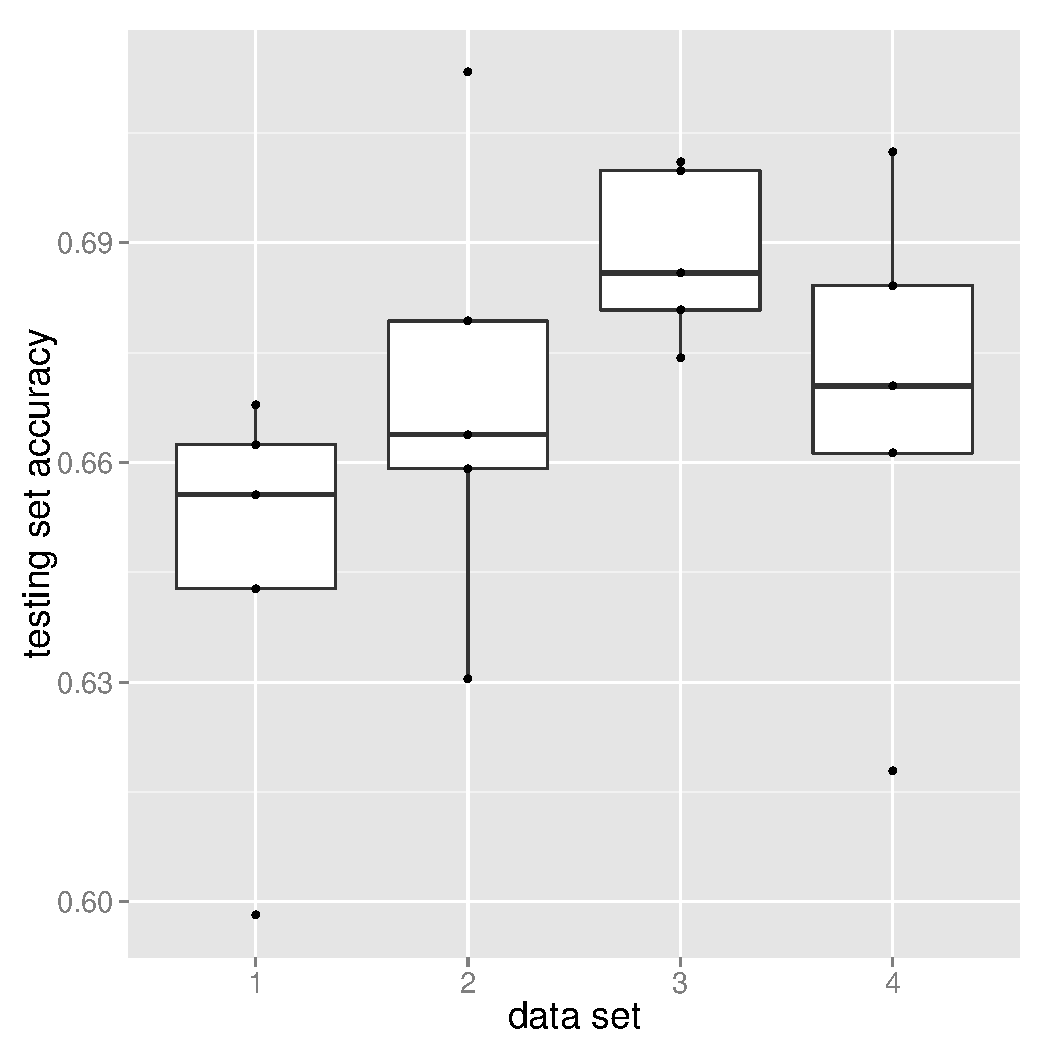
\includegraphics[width=0.34\paperwidth]{images/breast_cancer_08-accuracies-testing-bb_bu.pdf} & \includegraphics[width=0.34\paperwidth]{images/breast_cancer_08-accuracies-testing-by_cr.pdf}\tabularnewline
rma\_combat-data.pbtxt & mas5\_combat-data.pbtxt\tabularnewline
\includegraphics[width=0.34\paperwidth]{images/breast_cancer_08-accuracies-testing-ep_fi.pdf} & \includegraphics[width=0.34\paperwidth]{images/breast_cancer_08-accuracies-testing-fm_gf.pdf}\tabularnewline
\end{tabular}
\par\end{centering}
\caption[Box-plot for neural network prediction pre-trained with an autoencoder
on differently normalized data sets.]{\label{fig:accuracy-plots-for-breast_cancer_08}Box-plot for neural
network prediction pre-trained with an autoencoder on the 4 differently
normalized data sets rma-data.pbtxt, mas5-data.pbtxt, rma\_combat-data.pbtxt,
and mas5\_combat-data.pbtxt in breast\_cancer\_08. The box-plot shows
on the x-axis the 4 data sets, and on the y-axis the achieved accuracies
on the testing data set for each of the 5 repetitions.}
\end{figure}
The architecture of the classifier network was 500-1000-1. Figure
\ref{fig:accuracy-plots-for-breast_cancer_08} shows the resulting
accuracy box plots for the different normalizations. None of the plots
show a clear increasing accuracy from data set 1 to data set 4. However,
the silhouettes of the box-plots seem to show increasing accuracy.
``Silhouette'' means, for each data set, the interval from the accuracy
of the repetition with lowest to the accuracy of the repetition with
highest accuracy; or differently, the maximal outliers. In addition,
the median of the accuracies of data set 1 is smaller than the median
of the accuracies of both data set 3 and 4, for every normalization.
The fact that the median of the accuracies of data set 2 is not always
greater than the median of the accuracies of data set 1 could be due
to randomness in data subsampling when creating the 5 repetitions.
Another reason could be that the 28 additional unlabeled samples ($29-15=14$
label 0 samples, and 14 label 1 samples) provide little benefit to
a pre-trained classifier.

\subsubsection{Different Normalizations}

When comparing the accuracies yielded by the different normalizations
to each other, a table of the mean accuracies for each normalization
and data sets 1-4 is helpful. Table \ref{tab:Mean-accuracies-for-each-normalization}
shows the following:

\begin{table}
\begin{centering}
\begin{tabular}{|c||c|c|c|c|}
\hline 
normalization & \multicolumn{4}{c|}{data set}\tabularnewline
\hline 
 & 1 & 2 & 3 & 4\tabularnewline
\hline 
\hline 
rma & 0.65 & 0.67 & 0.69 & 0.67\tabularnewline
\hline 
mas5 & 0.58 & 0.58 & 0.63 & 0.61\tabularnewline
\hline 
mas5,log2 & 0.59 & 0.61 & 0.6 & 0.62\tabularnewline
\hline 
rma,combat & 0.61 & 0.61 & 0.62 & 0.61\tabularnewline
\hline 
mas5,combat & 0.60 & 0.59 & 0.63 & 0.64\tabularnewline
\hline 
mas5,log2,combat & 0.64 & 0.66 & 0.64 & 0.64\tabularnewline
\hline 
\end{tabular}
\par\end{centering}
\caption{\label{tab:Mean-accuracies-for-each-normalization}Mean accuracies
for each normalization and data set in breast\_cancer\_08.}
\end{table}
\begin{itemize}
\item RMA alone (i.e. without ComBat pre-processing) out-performs all other
tested combinations of normalization method and pre-processing in
all data sets tested.
\item Using ComBat as pre-processing leads to worse accuracies on the RMA-normalized
data, but improves accuracies when using MAS5 (except in data set
3).
\item RMA seems to perform consistently better than MAS5 without log2 (an
exception is data set 3 with ComBat pre-processing), but MAS5 with
log2 and ComBat perform better than RMA with ComBat (due to RMA taking
a performance hit when used together with ComBat).
\item Taking the log2 of MAS5-normalized data only improves accuracies when
the data is ComBat pre-processed.
\end{itemize}

\subsubsection{ZCA Normalization}

We also tried applying ZCA normalization after all 4 normalizations
tried above. This step helped in face recognition, for example \cite{KrizhevskyHinton2009}.
However, for our data set it resulted in random classifiers, i.e.
their accuracies were around 0.5.


\section{Comparison of SVM, TSVM, FFN, DBN\label{sec:breast_cancer_12}}

A problem in the design of the data sets of breast\_cancer\_08 is
that the number of label 0 and label 1 samples is not balanced. This
is due to the class imbalance in GSE25055 and GSE25065. The next data
set \index{breast_cancer_12@breast\_cancer\_12}breast\_cancer\_12
thus had balanced classes in the unlabeled training samples.

To be able to statistically detect a possible rise in accuracy with
a rising number of unlabeled samples, we also increased the number
of sub-sampling repetitions. Also, instead of using autoencoder or
RBM for pre-training, we used a Deep Belief Network.

\subsection{Data Set Design}

Following the same arguments as in creating data set breast\_cancer\_08,
we aimed for the following properties. All training/validation data
sets should have an equal number of 0/1 samples, otherwise \emph{deepnet}'s
predictions are biased towards the larger group. Samples used in the
unlabeled training/validation data set were also used for labeled
training/validation, otherwise there are not enough samples. Unlabeled
validation data sets were defined to be able to do model selection
during unsupervised training. As before, performance was measured
on the unseen test data sets.

There are the following differences between breast\_cancer\_12 and
breast\_cancer\_08. breast\_cancer\_12 includes an unlabeled validation
data set whose purpose is to be able to early-stop pre-training, which
was necessary for learning multiple hidden layers in a DBN. The only
normalization used was RMA (without ComBat), because it performed
best in data set breast\_cancer\_08. There are 20 instead of 5 repetitions
for each data set. Again the sub-sampling repetitions were made by
selecting the samples at random from the eligible samples. The labeled
samples were held constant across all 6 data sets within one repetition,
to be able to directly compare performance between e.g. data sets
1 and 3 within a repetition. The only difference between data sets
1 and 3 is the unlabeled pre-training data.

\begin{table}
\begin{centering}
\begin{tabular}{|c|c|c||c|c|c|c|c|c|}
\hline 
\multicolumn{3}{|c||}{data set} & 1 & 2 & 3 & 4 & 5 & 6\tabularnewline
\hline 
\hline 
\multirow{2}{*}{(labeled)} & \multirow{2}{*}{testing} & GSE25055 & 0\textbar{}0 & 0\textbar{}0 & 0\textbar{}0 & 0\textbar{}0 & 0\textbar{}0 & 0\textbar{}0\tabularnewline
\cline{3-9} 
 &  & GSE25065 & 42\textbar{}42 & 42\textbar{}42 & 42\textbar{}42 & 42\textbar{}42 & 42\textbar{}42 & 42\textbar{}42\tabularnewline
\hline 
\multirow{4}{*}{labeled} & \multirow{2}{*}{training} & GSE25055 & 10\textbar{}10 & 10\textbar{}10 & 10\textbar{}10 & 10\textbar{}10 & 10\textbar{}10 & 10\textbar{}10\tabularnewline
\cline{3-9} 
 &  & GSE25065 & 0\textbar{}0 & 0\textbar{}0 & 0\textbar{}0 & 0\textbar{}0 & 0\textbar{}0 & 0\textbar{}0\tabularnewline
\cline{2-9} 
 & \multirow{2}{*}{validation} & GSE25055 & 10\textbar{}10 & 10\textbar{}10 & 10\textbar{}10 & 10\textbar{}10 & 10\textbar{}10 & 10\textbar{}10\tabularnewline
\cline{3-9} 
 &  & GSE25065 & 0\textbar{}0 & 0\textbar{}0 & 0\textbar{}0 & 0\textbar{}0 & 0\textbar{}0 & 0\textbar{}0\tabularnewline
\hline 
\multirow{6}{*}{unlabeled} & \multirow{3}{*}{training} & GSE25055 & 0\textbar{}0 & 6\textbar{}6 & 12\textbar{}12 & 17\textbar{}17 & 23\textbar{}23 & 29\textbar{}29\tabularnewline
\cline{3-9} 
 &  & GSE25065 & 0\textbar{}0 & 4\textbar{}4 & 8\textbar{}8 & 13\textbar{}13 & 17\textbar{}17 & 21\textbar{}21\tabularnewline
\cline{3-9} 
 &  & $\sum_{Training}$ & 0\textbar{}0 & 10\textbar{}10 & 20\textbar{}20 & 30\textbar{}30 & 40\textbar{}40 & 50\textbar{}50\tabularnewline
\cline{2-9} 
 & \multirow{3}{*}{validation} & GSE25055 & 0\textbar{}0 & 6\textbar{}6 & 11\textbar{}11 & 17\textbar{}17 & 22\textbar{}22 & 28\textbar{}28\tabularnewline
\cline{3-9} 
 &  & GSE25065 & 0\textbar{}0 & 4\textbar{}4 & 9\textbar{}9 & 12\textbar{}12 & 17\textbar{}17 & 21\textbar{}21\tabularnewline
\cline{3-9} 
 &  & $\sum_{Validation}$ & 0\textbar{}0 & 10\textbar{}10 & 20\textbar{}20 & 29\textbar{}29 & 39\textbar{}39 & 49\textbar{}49\tabularnewline
\hline 
repeats &  &  & 20 & 20 & 20 & 20 & 20 & 20\tabularnewline
\hline 
\end{tabular}
\par\end{centering}
\caption[Data set design of breast\_cancer\_12.]{\label{tab:design-of-breast_cancer_12}Data set design of breast\_cancer\_12.
There are always 42\textbar{}42 testing samples. There is no overlap
between  unlabeled training,  unlabeled validation,  labeled training,
and  labeled validation samples. The number of labeled samples is
held constant at 20\textbar{}20 (10\textbar{}10 for training and validation)
across data sets. The number of training and validation samples is
almost equal in each data set (the difference is at most 1, for the
unlabeled data). The number of unlabeled samples is increased linearly
from 0\textbar{}0 to the maximum number of remaining samples 50\textbar{}50
(29\textbar{}29 in GSE25055 and 21\textbar{}21 in GSE25065). The labeled
data are equal across all data sets (but different between different
repetitions). ``repeats'' are the number of sub-samples drawn.}
\end{table}
Table \ref{tab:design-of-breast_cancer_12} shows the number of samples
used in the 6 data sets of breast\_cancer\_12.

\subsection{DBN Training}

breast\_cancer\_12\_aa - dv is like breast\_cancer\_08\_jh, except
that in pre-training the hidden layers, it uses the model performing
best on the validation data, not the model of the last training iteration.
This is possible because there is an unlabeled validation data set
in breast\_cancer\_12. In addition, instead of using RBMs or autoencoders,
DBNs were used for pre-training.

The architecture of the DBNs was 500-1000-1000-2000-1, that means
the input layer has 500 nodes for the 500 most significant genes,
then there are three hidden layers with sizes 1000, 1000, and 2000,
and the output layer has 1 node which outputs the probability that
the input sample has label 1.

We reduced the unsupervised learning rate from ``base\_epsilon: 0.01''
to 0.001, and increased ``sparsity\_damping: 0.9'' to 0.99 in layer
2 and 3. We do this because otherwise these layers have their best
model on the labeled validation data set very early in training, and
also sometimes ``explode''\footnote{A network ``explodes'' when its parameters (weights and biases)
and reconstruction error oscillate. This happens because neural network
training is a gradient descent method, with the size of the gradient
decent step depending on the learning rate and the sparsity meta-parameters
(refer to section \ref{subsec:Sparsity-Target}). A too large step
can cause the network's error to get worse.}.

Another difference is that the supervised learning rate in breast\_cancer\_12\_aa
- dv is 0.0001, not 0.001. \cite{SrivastavaSalakhutdinov2014} says
that when choosing the learning rate smaller than the best learning
rate for randomly initialized nets, the information in the pretrained
weights seems to be retained, and finetuning improves the final generalization
error compared to not using dropout when finetuning.

We also changed ``eval\_after: 500'' to 100 in train\_supervised.pbtxt,
in order to check more often for the optimal solution, because supervised
training sometimes finds the best model on the validation data set
very early in training.

Deep Belief Networks need unlabeled samples during pre-training. Thus,
data set 1, which does not contain unlabeled samples, cannot be used
to train DBNs. Therefore we trained DBNs only on data sets 2 to 6.

\subsection{Using Both Training and Validation Data Sets for Training TSVMs}

To predict using TSVM, for every repetition and every data set, we
joined labeled training, labeled validation data, unlabeled training,
and unlabeled validation data to the training input file to be used
by TSVM. This was done to be fair to TSVM, because deepnet also has
access to these labeled and unlabeled samples. The testing data set
was the same as that used for the neural networks.

\subsection{Comparison of Neural Networks with Support Vector Machines\label{subsec:Comparison-of-Neuronal-Networks-with-Support-Vector-Machines}}

\begin{figure}
\begin{centering}
\begin{tabular}{cc}
(a) FFN & (b) DBN\tabularnewline
\includegraphics[width=0.34\paperwidth]{images/breast_cancer_12-ffn-accuracies-testing-fa_ft.pdf} & \includegraphics[width=0.34\paperwidth]{images/breast_cancer_12-dbn-accuracies-testing-aa_dv.pdf}\tabularnewline
(c) SVM & (d) TSVM\tabularnewline
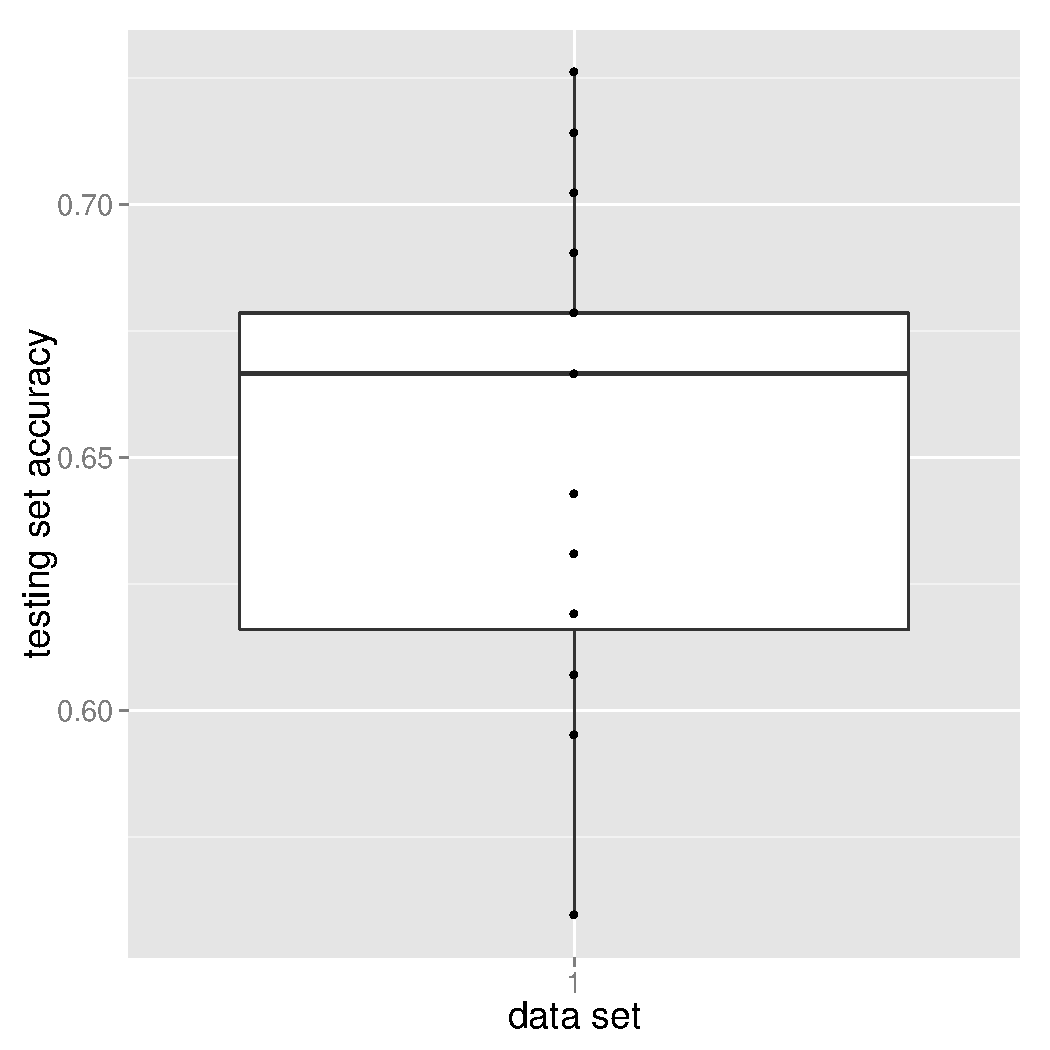
\includegraphics[width=0.34\paperwidth]{images/breast_cancer_12-svm-accuracies-learn-training_validation.pdf} & 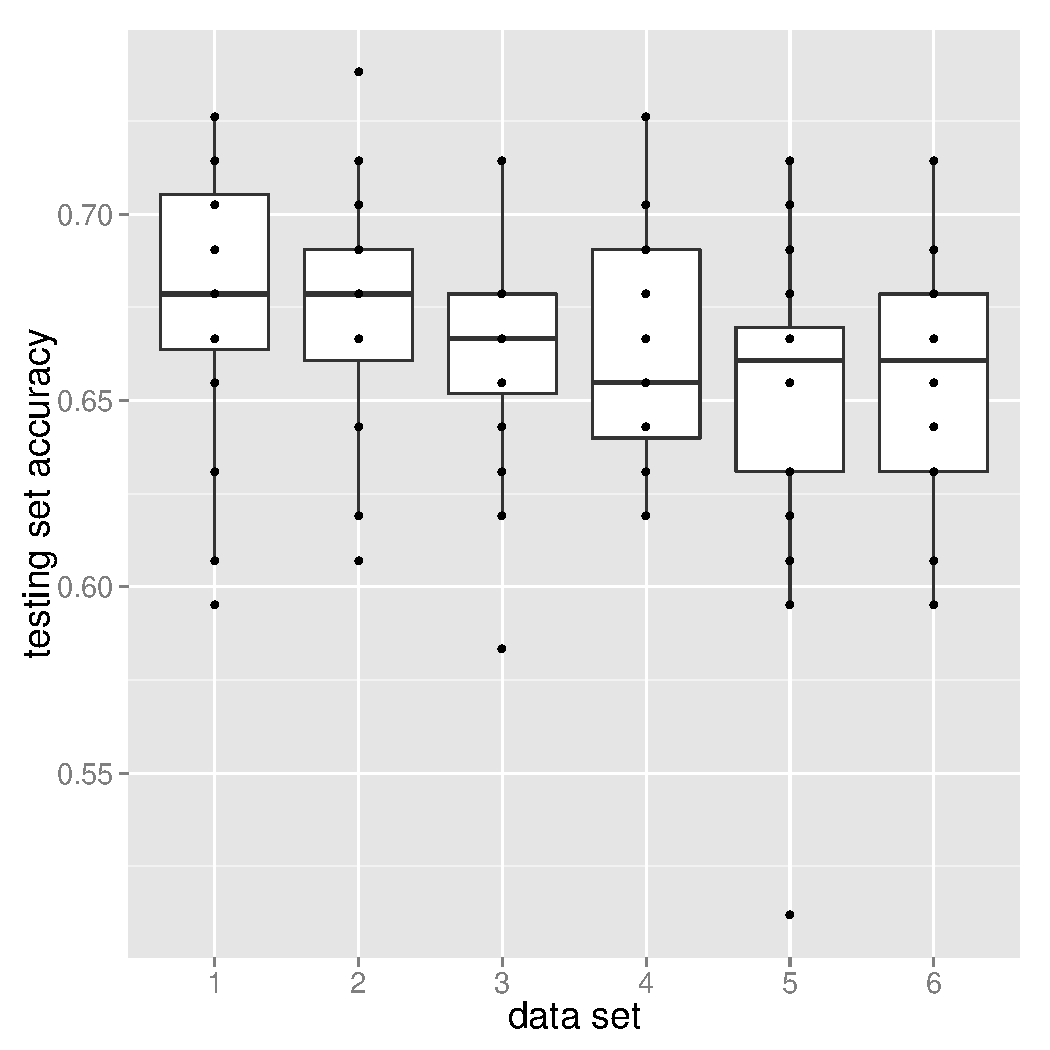
\includegraphics[width=0.34\paperwidth]{images/breast_cancer_12-svmlight-accuracies-learn_training_validation.pdf}\tabularnewline
\end{tabular}
\par\end{centering}
\caption[Accuracy comparison of supervised feed-forward network, semi-supervised
Deep Belief Network, supervised support vector machine, and semi-supervised
transductive support vector machine.]{\label{fig:Accuracy-comparison-of-breast_cancer_12}Accuracy comparison
of (a) supervised feed-forward network, (b) semi-supervised Deep Belief
Network, (c) supervised support vector machine, and (d) semi-supervised
transductive support vector machine. On the x-axis of each plot are
the sub-data-sets (of breast\_cancer\_12) predicted for each algorithm,
on the y-axis is the accuracy.}
\end{figure}

\paragraph{Paired and Two-Sided Wilcoxon Test}

Figure \ref{fig:Accuracy-comparison-of-breast_cancer_12} shows that
there is no clear improvement by increasing the number of unlabeled
samples, neither when using a DBN, nor a TSVM.

This can be quantified using a paired and two-sided Wilcoxon test\index{Wilcoxon test}.
It is paired over the repetitions because the labeled training and
validation sets are constant across data sets 1-6 within a repetition
and the only difference is the amount of unlabeled data used during
training. It is two-sided because we do not know before the experiment
which algorithm on a data set will perform better than another. The
null hypothesis is that the true accuracy shift between the two compared
experiments is zero.

By experiment we mean the set of accuracies in figure \ref{fig:Accuracy-comparison-of-breast_cancer_12}
when keeping the prediction method and sub-data-set of breast\_cancer\_12
constant, but varying the repetition. Hence there are 1 FFN, 5 DBN,
1 SVM, and 6 TSVM experiments.

We could now compare all experiments against all other experiments
using a Wilcoxon test. However, this would be ``fishing for significance'',
and we would have to correct the p-values for multiple testing. If
comparing all against all, there are $(1+5+1+6)*(1+5+1+6-1)/2=78$
comparisons, and we would lose a lot of power due to comparisons that
are not interesting. That is why we only compare the experiments in
figure \ref{fig:Accuracy-comparison-of-breast_cancer_12} row-wise
and column-wise, because these comparisons allow an interpretation.
That way there are only $1*5+1*6+1*1+5*6=42$ comparisons. We adjust
the p-values within each comparison only.

\subsubsection{Comparison of FFN With DBN}

Table \ref{tab:breast_cancer_12-FFN-versus-DBN} compares a supervised
Feed-Forward Network (FFN) against a semi-supervised Deep Belief Network
(DBN). Because the FFN is trained supervisedly, it cannot be trained
on data sets 2-6, which contain unlabeled samples.

\begin{table}[p]
\begin{centering}
\begin{tabular}{|c|c|c|c|c|c|c|c|c|}
\hline 
n1 & method1 & n2 & method2 & p\_value & estimate & ci\_lower & ci\_upper & p\_adjust\tabularnewline
\hline 
\hline 
1 & FFN & 2 & DBN & 0.896 & 0.000 & -0.007 & 0.009 & 0.955\tabularnewline
\hline 
1 & FFN & 3 & DBN & 0.255 & 0.005 & -0.004 & 0.013 & 0.637\tabularnewline
\hline 
1 & FFN & 4 & DBN & 0.723 & 0.001 & -0.009 & 0.009 & 0.955\tabularnewline
\hline 
1 & FFN & 5 & DBN & 0.255 & 0.004 & -0.003 & 0.011 & 0.637\tabularnewline
\hline 
1 & FFN & 6 & DBN & 0.955 & 0.000 & -0.010 & 0.007 & 0.955\tabularnewline
\hline 
\end{tabular}
\par\end{centering}
\caption[Comparison of FFN with DBN.]{\label{tab:breast_cancer_12-FFN-versus-DBN}Comparison of FFN with
DBN. Columns \emph{n1} and \emph{n2} are the sub-data-set indices
to be compared. (A higher index means means this sub-data-set has
more unlabeled samples than a lower index.) \emph{method1} and \emph{method2}
are the methods to be compared. \emph{p\_value} is the unadjusted
p-value, \emph{estimate} is the estimated difference in accuracy of
the comparison (e.g. 0.1 would mean method1's accuracy is better by
an estimated 10 percent points), \emph{ci\_lower} and \emph{ci\_upper}
are the lower and upper confidence interval for the estimated accuracy
difference. \emph{p\_adjust} is the p-value corrected for multiple
testing. Raw and adjusted p-values below 5\% are written in bold font.}
\end{table}

The lowest adjusted p-value is 0.637, which means there is no significant
difference between FFN and DBN.

\subsubsection{Comparison of SVM With TSVM}

Table \ref{tab:breast_cancer_12-SVM-versus-TSVM} compares a supervised
Support Vector Machine (SVM) against a semi-supervised Transductive
Support Vector Machine (TSVM). Because the SVM is trained supervisedly,
it cannot be trained on data sets 2-6, which contain unlabeled samples.

\begin{table}[p]
\begin{centering}
\begin{tabular}{|c|c|c|c|c|c|c|c|c|}
\hline 
n1 & method1 & n2 & method2 & p\_value & estimate & ci\_lower & ci\_upper & p\_adjust\tabularnewline
\hline 
\hline 
1 & SVM & 1 & TSVM & \textbf{0.026} & -0.024 & -0.054 & 0.000 & 0.158\tabularnewline
\hline 
1 & SVM & 2 & TSVM & 0.104 & -0.018 & -0.042 & 0.006 & 0.313\tabularnewline
\hline 
1 & SVM & 3 & TSVM & 0.240 & -0.012 & -0.042 & 0.012 & 0.359\tabularnewline
\hline 
1 & SVM & 4 & TSVM & 0.191 & -0.012 & -0.036 & 0.012 & 0.359\tabularnewline
\hline 
1 & SVM & 5 & TSVM & 0.779 & 0.000 & -0.030 & 0.024 & 0.779\tabularnewline
\hline 
1 & SVM & 6 & TSVM & 0.588 & -0.006 & -0.024 & 0.018 & 0.706\tabularnewline
\hline 
\end{tabular}
\par\end{centering}
\caption[Comparison of SVM with TSVM.]{\label{tab:breast_cancer_12-SVM-versus-TSVM}Comparison of SVM with
TSVM. See table \ref{tab:breast_cancer_12-FFN-versus-DBN} for the
legend.}
\end{table}

The lowest adjusted p-value is 0.158 between SVM and TSVM on data
set 1.

\subsubsection{Comparison of FFN With SVM}

Table \ref{fig:breast_cancer_12-FFN-versus-SVM} compares a non-linear
Feed-Forward Network against a Support Vector Machine with linear
kernel. Both algorithms are supervised.

\begin{table}[p]
\begin{centering}
\begin{tabular}{|c|c|c|c|c|c|c|c|c|}
\hline 
n1 & method1 & n2 & method2 & p\_value & estimate & ci\_lower & ci\_upper & p\_adjust\tabularnewline
\hline 
\hline 
1 & FFN & 1 & SVM & 0.926 & -0.003 & -0.023 & 0.021 & 0.926\tabularnewline
\hline 
\end{tabular}
\par\end{centering}
\caption[Comparison of FFN with SVM.]{\label{fig:breast_cancer_12-FFN-versus-SVM}Comparison of FFN with
SVM. See table \ref{tab:breast_cancer_12-FFN-versus-DBN} for the
legend.}
\end{table}

The p-value is 0.926 and not significant.

\subsubsection{Comparison of DBN With TSVM}

Table \ref{tab:breast_cancer_12-TSVM-versus-DBN} compares a non-linear
Deep Belief Network against a Transductive Support Vector Machine
with linear kernel. Both algorithms are semi-supervised.

\begin{table}[p]
\begin{centering}
\begin{tabular}{|c|c|c|c|c|c|c|c|c|}
\hline 
n1 & method1 & n2 & method2 & p\_value & estimate & ci\_lower & ci\_upper & p\_adjust\tabularnewline
\hline 
\hline 
1 & TSVM & 2 & DBN & \textbf{0.002} & 0.023 & 0.009 & 0.043 & \textbf{0.012}\tabularnewline
\hline 
1 & TSVM & 3 & DBN & \textbf{0.000} & 0.031 & 0.018 & 0.044 & \textbf{0.004}\tabularnewline
\hline 
1 & TSVM & 4 & DBN & \textbf{0.000} & 0.025 & 0.014 & 0.037 & \textbf{0.004}\tabularnewline
\hline 
1 & TSVM & 5 & DBN & \textbf{0.000} & 0.029 & 0.018 & 0.040 & \textbf{0.004}\tabularnewline
\hline 
1 & TSVM & 6 & DBN & \textbf{0.001} & 0.027 & 0.013 & 0.043 & \textbf{0.011}\tabularnewline
\hline 
2 & TSVM & 2 & DBN & 0.065 & 0.020 & -0.001 & 0.043 & 0.129\tabularnewline
\hline 
2 & TSVM & 3 & DBN & \textbf{0.009} & 0.023 & 0.006 & 0.039 & \textbf{0.047}\tabularnewline
\hline 
2 & TSVM & 4 & DBN & \textbf{0.016} & 0.021 & 0.005 & 0.036 & 0.060\tabularnewline
\hline 
2 & TSVM & 5 & DBN & \textbf{0.016} & 0.022 & 0.005 & 0.038 & 0.060\tabularnewline
\hline 
2 & TSVM & 6 & DBN & \textbf{0.029} & 0.022 & 0.003 & 0.040 & 0.087\tabularnewline
\hline 
3 & TSVM & 2 & DBN & 0.113 & 0.016 & -0.003 & 0.035 & 0.199\tabularnewline
\hline 
3 & TSVM & 3 & DBN & \textbf{0.050} & 0.017 & 0.000 & 0.036 & 0.115\tabularnewline
\hline 
3 & TSVM & 4 & DBN & \textbf{0.035} & 0.016 & 0.004 & 0.029 & 0.095\tabularnewline
\hline 
3 & TSVM & 5 & DBN & \textbf{0.024} & 0.017 & 0.003 & 0.031 & 0.080\tabularnewline
\hline 
3 & TSVM & 6 & DBN & \textbf{0.042} & 0.014 & 0.001 & 0.030 & 0.105\tabularnewline
\hline 
4 & TSVM & 2 & DBN & 0.211 & 0.012 & -0.009 & 0.035 & 0.333\tabularnewline
\hline 
4 & TSVM & 3 & DBN & 0.070 & 0.018 & -0.001 & 0.032 & 0.132\tabularnewline
\hline 
4 & TSVM & 4 & DBN & 0.131 & 0.013 & -0.003 & 0.026 & 0.218\tabularnewline
\hline 
4 & TSVM & 5 & DBN & 0.059 & 0.014 & -0.001 & 0.030 & 0.127\tabularnewline
\hline 
4 & TSVM & 6 & DBN & 0.225 & 0.011 & -0.006 & 0.028 & 0.338\tabularnewline
\hline 
5 & TSVM & 2 & DBN & 0.614 & 0.005 & -0.018 & 0.029 & 0.658\tabularnewline
\hline 
5 & TSVM & 3 & DBN & 0.467 & 0.007 & -0.013 & 0.025 & 0.538\tabularnewline
\hline 
5 & TSVM & 4 & DBN & 0.422 & 0.007 & -0.011 & 0.021 & 0.533\tabularnewline
\hline 
5 & TSVM & 5 & DBN & 0.444 & 0.007 & -0.011 & 0.024 & 0.533\tabularnewline
\hline 
5 & TSVM & 6 & DBN & 0.641 & 0.003 & -0.014 & 0.021 & 0.663\tabularnewline
\hline 
6 & TSVM & 2 & DBN & 0.514 & 0.006 & -0.012 & 0.025 & 0.571\tabularnewline
\hline 
6 & TSVM & 3 & DBN & 0.380 & 0.006 & -0.006 & 0.020 & 0.519\tabularnewline
\hline 
6 & TSVM & 4 & DBN & 0.444 & 0.005 & -0.011 & 0.018 & 0.533\tabularnewline
\hline 
6 & TSVM & 5 & DBN & 0.360 & 0.006 & -0.009 & 0.021 & 0.515\tabularnewline
\hline 
6 & TSVM & 6 & DBN & 0.896 & 0.001 & -0.012 & 0.017 & 0.896\tabularnewline
\hline 
\end{tabular}
\par\end{centering}
\caption[Comparison of DBN with TSVM.]{\label{tab:breast_cancer_12-TSVM-versus-DBN}Comparison of DBN with
TSVM. See table \ref{tab:breast_cancer_12-FFN-versus-DBN} for the
legend.}
\end{table}

Due to their p-values being smaller than 5\%, we can conclude that
the TSVM on data set 1 is significantly better than the DBN on all
data sets. In addition, the SVM on data set 2 is significantly better
than the DBN on data set 3. For example, the TSVM trained on sub-data-set
1 is better than the DBN trained on sub-data-set 2 by 2.3 percent
points in accuracy.

The result that the TSVM on data set 1 is better than the DBNs, and
not on data set 5 or 6, which consist of more unlabeled data, is contrary
to the expected hypothesis that a semi-supervised TSVM trained on
more unlabeled samples is better than one on less unlabeled samples.

The table also shows that the advantage of using a TSVM over a DBN
becomes negligible when adding more unlabeled data to training. (The
``estimate'' value declines with increasing data set, from 2.0\%
on data set 2 versus data set 2 to 0.1\% on data set 6 versus data
set 6.)

\subsubsection{Comparison of TSVM With TSVM}

The largest differences in prediction accuracy are within TSVM. Due
to it being semi-supervised we were interested in whether there are
significant accuracy differences within the sub-data-sets of breast\_cancer\_12.
Table \ref{tab:breast_cancer_12-TSVM-versus-TSVM} compares all TSVMs
on the sub-data-sets against all other TSVM on the sub-data-sets.

\begin{table}
\begin{centering}
\begin{tabular}{|c|c|c|c|c|c|c|c|c|}
\hline 
n1 & method1 & n2 & method2 & p\_value & estimate & ci\_lower & ci\_upper & p\_adjust\tabularnewline
\hline 
\hline 
1 & TSVM & 2 & TSVM & 0.254 & 0.012 & -0.012 & 0.030 & 0.347\tabularnewline
\hline 
1 & TSVM & 3 & TSVM & 0.184 & 0.018 & -0.006 & 0.036 & 0.320\tabularnewline
\hline 
1 & TSVM & 4 & TSVM & 0.061 & 0.018 & 0.000 & 0.036 & 0.182\tabularnewline
\hline 
1 & TSVM & 5 & TSVM & \textbf{0.023} & 0.030 & 0.006 & 0.048 & 0.113\tabularnewline
\hline 
1 & TSVM & 6 & TSVM & \textbf{0.007} & 0.030 & 0.012 & 0.048 & \textbf{0.098}\tabularnewline
\hline 
2 & TSVM & 3 & TSVM & 0.588 & 0.006 & -0.006 & 0.024 & 0.679\tabularnewline
\hline 
2 & TSVM & 4 & TSVM & 0.222 & 0.012 & -0.006 & 0.024 & 0.332\tabularnewline
\hline 
2 & TSVM & 5 & TSVM & \textbf{0.015} & 0.018 & 0.006 & 0.030 & 0.110\tabularnewline
\hline 
2 & TSVM & 6 & TSVM & \textbf{0.031} & 0.024 & 0.006 & 0.030 & 0.115\tabularnewline
\hline 
3 & TSVM & 4 & TSVM & 0.759 & 0.000 & -0.012 & 0.018 & 0.813\tabularnewline
\hline 
3 & TSVM & 5 & TSVM & 0.192 & 0.012 & -0.006 & 0.024 & 0.320\tabularnewline
\hline 
3 & TSVM & 6 & TSVM & 0.154 & 0.012 & -0.006 & 0.030 & 0.320\tabularnewline
\hline 
4 & TSVM & 5 & TSVM & 0.313 & 0.012 & -0.012 & 0.030 & 0.391\tabularnewline
\hline 
4 & TSVM & 6 & TSVM & 0.110 & 0.012 & 0.000 & 0.024 & 0.274\tabularnewline
\hline 
5 & TSVM & 6 & TSVM & 0.977 & 0.000 & -0.024 & 0.018 & 0.977\tabularnewline
\hline 
\end{tabular}
\par\end{centering}
\caption[Comparison of TSVM with TSVM on different numbers of unlabeled samples.]{\label{tab:breast_cancer_12-TSVM-versus-TSVM}Comparison of TSVM
with TSVM on different numbers of unlabeled samples. See table \ref{tab:breast_cancer_12-FFN-versus-DBN}
for the legend. Duplicate rows were removed.}
\end{table}

The lowest adjusted p-value is 0.098 between data set 1 and data set
6. Again, this is contrary to the expected hypothesis that adding
unlabeled data in the training of the semi-supervised TSVM is beneficial
to its prediction accuracy.

\section{Less Network Parameters\label{sec:breast_cancer_15}}

Since breast\_cancer\_12 has a negative result in summary, because
it cannot confirm the benefit of adding unlabeled samples to training,
in data set \index{breast_cancer_15@breast\_cancer\_15}breast\_cancer\_15
we considered the differences in data sources and artificial neural
network configurations between our and the ones in image recognition,
where DBNs are successful. We also increased the number of input genes
from the 500 most variable genes used as input genes in previous data
sets to all 22,283 available genes.

\subsection{Too Many Free Parameters}

\cite{HintonTeh2006} write that they use a 3-hidden-layer network
with about $1.7*10^{6}$ weights. They used 44000 training samples
with 28{*}28 pixels each. So altogether they have about 34.5 million
``training numbers'', and 1.7 million weights that have to be determined.
Precisely, their ratio of input numbers to number of weights is 
\begin{eqnarray*}
\frac{\mbox{input numbers}}{\mbox{weights}} & = & \frac{44000*28*28}{28*28*500+500*500+500*2000+2000*10}\approx20.8.
\end{eqnarray*}

In contrast to that we have (in data set breast\_cancer\_12, data
set 6) 238 training and validation samples, each of which has 500
expression levels, i.e. $238*500=119,000$ ``training numbers''
used totally in the input. The breast\_cancer\_12 artificial neural
networks all have an architecture of 500-1000-1000-2000-1 (500 input
nodes, 1000 hidden layer 1 nodes, 1000 hidden layer 2 nodes, 2000
hidden layer 3 nodes, and 1 output layer node). Hence, there are $500*1000+1000*1000+1000*2000+2000*1\approx3.5*10^{6}$
weights to be learnt. The ratio of $\frac{\mbox{input numbers}}{\mbox{weights}}\approx0.034\ll20.8$
is much lower in our case than in the image recognition case. 

This can be changed by using all $i=22,283$ genes as inputs, and
only a very small number of hidden nodes $h$ (assuming for simplicity
that all hidden layers have the same number of nodes). If we take
$i=22,283$, and there are 238 training samples (in fact we have only
20 labeled plus 100 unlabeled training samples in breast\_cancer\_12),
then we have $22,283*238=5,303,354$ measured numbers. The ratio formula
is
\begin{eqnarray*}
r(h) & = & \frac{22283*238}{22283*h+h*h+h*h+h*o},
\end{eqnarray*}
where $h$ is the number of hidden nodes and $o$ is the number of
output samples and is equal to 1, because the labeled cases have a
binary label.

\subsection{Data Set Design\label{subsec:Data-Set-Design-of-breast_cancer_15}}

To exclude that a batch effect between GSE25055 and GSE25065 negatively
affects semi-supervised learning, in breast\_cancer\_15 we only use
GSE25055, also for testing. Again we use 10\textbar{}10 labeled training
and validation samples. This leaves us with remaining $57-20=37$
label 1 samples for testing, and we also use 37 label 0 samples. Like
in previous data sets, all samples for the labeled training and validation
data sets can be re-used in the unlabeled data set, because the labels
are not given to the neural network during pre-training.

We choose a reasonably large unlabeled validation data set of 28 samples
like in breast\_cancer\_12 (although in breast\_cancer\_12 we used
21 GSE25065 samples in addition). The ratio of label 0 to label 1
samples is $249/57\approx4.37$. To have a sufficient number of label
1 unlabeled validation samples, we use $100|25$ (where $x|y$ means
$x$ label 0 samples and $y$ label 1 samples) unlabeled validation
samples, where the 25 label 1 samples are replicated 4 times (written
$100|25*4$). This leaves $57-25=32$ label 1 samples for the unlabeled
training data set. Replicating label 1 samples 4 times in the data
set to have the same ratio of different label 0 and label 1 samples
as in the unlabeled validation data set gives $128|32*4=128|128$
samples.

Altogether, there are in the labeled and unlabeled training data $10|10+128|32*4=138|138$
samples = 276 samples, when counting the quadrupled label 1 samples
as 4 individual samples. When counting the quadrupled samples as only
1 real sample, there are $10|10+128|32=10*2+128+32=180$ samples.
So $t_{quad}=276$, $t_{indiv}=180$, $o=1$.

The ratio is then 
\begin{eqnarray*}
r(h,t) & = & \frac{22283*t}{22283*h+h*h+h*h+h*o}.
\end{eqnarray*}
For a hidden layer size of $h=10$, $r(h,t)$ is shown in table \ref{tab:breast_cancer_12-number-r}
for the 6 different data sets (containing an increasing number of
samples $t$).
\begin{table}
\begin{centering}
\begin{tabular}{|c||c|c|c|c|c|c|}
\hline 
data set & 1 & 2 & 3 & 4 & 5 & 6\tabularnewline
\hline 
\hline 
$t_{quad}$ & 2{*}10 & 2{*}(10+24) & 2{*}(10+52) & 2{*}(10+76) & 2{*}(10+104) & 2{*}(10+128)\tabularnewline
\hline 
$r(10,t_{quad})$ & 2.00 & 6.79 & 12.39 & 17.18 & 22.78 & 27.57\tabularnewline
\hline 
$t_{indiv}$ & 2{*}10 & 20+24+6 & 20+52+13 & 20+76+19 & 20+104+26 & 20+128+32\tabularnewline
\hline 
$r(10,t_{indiv})$ & 2.00 & 5.00 & 8.49 & 11.49 & 14.99 & 17.98\tabularnewline
\hline 
\end{tabular}
\par\end{centering}
\caption[The ratio of training samples to network parameters for 10 hidden
nodes.]{\label{tab:breast_cancer_12-number-r}The ratio of training samples
to network parameters, $r$,  for 10 hidden nodes in data set breast\_cancer\_15.
$t_{quad}$ is the number of samples when counting quadrupled samples
as 4 samples. $t_{indiv}$ is the number of samples when quadrupled
samples are counted as 1 sample.}
\end{table}
As the values for $r$ in the table are around 20 (for data set 6),
both for $t_{quad}$ and $t_{indiv}$, we choose a hidden layer node
size $h=10$. The architecture for the artificial neural networks
of breast\_cancer\_15 is 22283-10-10-10-1.

Another big change compared to previous data sets is the use of all
22,283 genes as input instead of only the 500 most variable genes.

The complete data set is shown in table \ref{tab:design-of-breast_cancer_15}.

\begin{table}
\begin{centering}
\begin{tabular}{|c|c|c||c|c|c|c|c|c|}
\hline 
\multicolumn{3}{|c||}{data set} & 1 & 2 & 3 & 4 & 5 & 6\tabularnewline
\hline 
\hline 
\multirow{6}{*}{\begin{turn}{90}
labeled
\end{turn}} & \multirow{2}{*}{testing} & GSE25055 & \multicolumn{6}{c|}{37\textbar{}37}\tabularnewline
\cline{3-9} 
 &  & GSE25065 & \multicolumn{6}{c|}{0\textbar{}0}\tabularnewline
\cline{2-9} 
 & \multirow{2}{*}{training} & GSE25055 & \multicolumn{6}{c|}{10\textbar{}10}\tabularnewline
\cline{3-9} 
 &  & GSE25065 & \multicolumn{6}{c|}{0\textbar{}0}\tabularnewline
\cline{2-9} 
 & \multirow{2}{*}{validation} & GSE25055 & \multicolumn{6}{c|}{10\textbar{}10}\tabularnewline
\cline{3-9} 
 &  & GSE25065 & \multicolumn{6}{c|}{0\textbar{}0}\tabularnewline
\hline 
\multirow{6}{*}{\begin{turn}{90}
unlabeled
\end{turn}} & \multirow{3}{*}{training} & GSE25055 & 0\textbar{}0 & 24\textbar{}6{*}4 & 52\textbar{}13{*}4 & 76\textbar{}19{*}4 & 104\textbar{}26{*}4 & 128\textbar{}32{*}4\tabularnewline
\cline{3-9} 
 &  & GSE25065 & \multicolumn{6}{c|}{0\textbar{}0}\tabularnewline
\cline{3-9} 
 &  & $\sum_{Training}$ & 0\textbar{}0 & 24\textbar{}6{*}4 & 52\textbar{}13{*}4 & 76\textbar{}19{*}4 & 104\textbar{}26{*}4 & 128\textbar{}32{*}4\tabularnewline
\cline{2-9} 
 & \multirow{3}{*}{validation} & GSE25055 & 0\textbar{}0 & 20\textbar{}5{*}4 & 40\textbar{}10{*}4 & 60\textbar{}15{*}4 & 80\textbar{}20{*}4 & 100\textbar{}25{*}4\tabularnewline
\cline{3-9} 
 &  & GSE25065 & \multicolumn{6}{c|}{0\textbar{}0}\tabularnewline
\cline{3-9} 
 &  & $\sum_{Validation}$ & 0\textbar{}0 & 20\textbar{}5{*}4 & 40\textbar{}10{*}4 & 60\textbar{}15{*}4 & 80\textbar{}20{*}4 & 100\textbar{}25{*}4\tabularnewline
\hline 
\multicolumn{3}{|c||}{repeats} & 20 & 20 & 20 & 20 & 20 & 20\tabularnewline
\hline 
\end{tabular}
\par\end{centering}
\caption[Data set design of breast\_cancer\_15.]{\label{tab:design-of-breast_cancer_15}Data set design of breast\_cancer\_15.
It contains 37\textbar{}37 labeled testing, 10\textbar{}10 labeled
training, 10\textbar{}10 labeled validation, $128|32*4$ unlabeled
training, and $100|25*4$ unlabeled validation samples (where $x|y*f$
means $x$ label 0 samples, and $y$ label 1 samples duplicated $f$
times). 6 sub-data-sets are created, with the first one having no
unlabeled data at all, the last one having $128|32*4$ training and
$100|25*4$ validation samples, and interpolated numbers in-between.
The labeled data are equal across all data sets (but different between
different repetitions). There are 20 sub-sampling repeats per sub-data-set.
All samples are from GSE25055, to avoid a possible batch-effect.}
\end{table}

\subsubsection{Different Training Parameters}

In comparison to breast\_cancer\_12, the unsupervised learning rate
(\emph{base\_epsilon}) was decreased from 0.01 to 0.001 for the pre-training
of hidden layer 1, and from 0.001 to 0.0001 for pre-training hidden
layers 2 and 3. We also changed the mini-batch\footnote{In training, the network parameters' deltas are alternatingly computed,
then the parameters are updated. (See equation \ref{eq:backpropagation-deltas}
in backpropagation training.) The mini-batch is the number of samples
whose deltas are accumulated before the network parameters are updated.} size from 100 to 1000, which leads to slower training, but iterates
over all training samples before changing weights, and thus approximates
the derivative of the weights more faithfully.

\subsection{Accuracy of DBN Fine-tuned with Back-propagation}

\begin{figure}
\begin{centering}
\includegraphics[width=0.68\columnwidth]{images/breast_cancer_15-accuracies-testing-aa_dv.pdf}
\par\end{centering}
\caption[Test set accuracies for different data sets with more and more unlabeled
training samples in a DBN on breast\_cancer\_15.]{\label{fig:Accuracy-in-breast_cancer_15}Box plots of test set accuracies
for different data sets with more and more unlabeled training samples
in a neural network pre-trained with DBN on breast\_cancer\_15. The
x-axis is the data sets in the order of rising number of unlabeled
samples; the y-axis is the test set accuracy. Data set 1 cannot be
used in DBNs because it does not contain unlabeled data. The y-axis
is the accuracy. Each dot represents the accuracy on a repetition.}
\end{figure}

Figure \ref{fig:Accuracy-in-breast_cancer_15} shows the accuracies
obtained for data set breast\_cancer\_15. The accuracies are better
than those obtained in breast\_cancer\_12: The median accuracy is
near 0.7 for all data sets except data set 3, while it was slightly
above 0.65 in breast\_cancer\_12. This may be due to less overfitting
because there are less model parameters, but it may also be due to
the training having used more input data (22,283 genes instead of
the 500 most significant).

To check whether there is a dependence of accuracies on the amount
of unlabeled samples available to training, we use a paired (over
the repetitions) and two-sided Wilcoxon test. The p-value for the
accuracy difference between data sets 2 and 6 is 0.089. The estimated
difference between accuracies of data sets 2 and 6 is 2.8 percent
points (0.028). (The 95\% confidence interval for the difference is
{[}-0.46; 6.7{]} percent points.) This shows a slight dependence of
accuracy on the number of unlabeled samples.

\subsection{TSVM Accuracies}

A TSVM was trained on the training and validation data of each repetition
of all data sets in breast\_cancer\_15. Figure \ref{fig:Accuracy-box-plots-of-breast_cancer_15}
shows the accuracies on the test sets. Inexplicably, training failed
in data set 2. Except for data set 2, one can see a slight accuracy
increase from data set 1 to data set 6, i.e. from the data set with
no unlabeled samples to the data set with the most unlabeled samples.
The accuracy difference between data sets 1 and 6 was tested for significance
with a paired (over the repetitions) and two-sided Wilcoxon test.
It is significant with a p-value of 0.0029, and the accuracy difference
between data sets 1 and 6 is an estimated 3.38 percent points (0.0338),
while its 95\% confidence interval is {[}2.02; 6.08{]} percent points.
Thus, in breast\_cancer\_15, the TSVM succeeded in increasing accuracy
slightly by learning from unlabeled samples.

When training a TSVM only on the training data (but leaving away the
validation data), in addition to data set 2, also data set 3 fails
to train a proper model with almost all their accuracies at 0.5, and
data set 4 has a median accuracy of only $\approx$0.575 (data not
shown). This may show that semi-supervised training using a TSVM fails
when not a sufficient number of unlabeled training samples is available.
Training the TSVM (supervisedly) using data set 1 did not fail.

\begin{figure}
\begin{centering}
\includegraphics[width=0.68\columnwidth]{images/breast_cancer_15-accuracies-svmlight.pdf}
\par\end{centering}
\caption[TSVM accuracies box plots on data set breast\_cancer\_15.]{\label{fig:Accuracy-box-plots-of-breast_cancer_15}TSVM accuracies
box plots on data set breast\_cancer\_15. On the x-axis are the data
sets in order of increasing number of unlabeled samples. On the y-axis
are the accuracies. Each dot is the accuracy of a repetition of a
data set of breast\_cancer\_15.}
\end{figure}

